\sloppy
\documentclass[14pt,a4paper,oneside]{extarticle}	% Размер основного шрифта и формата листа
\usepackage{xltxtra}						% Используется для вывода логотипа XeLaTeX
\usepackage{xunicode}						% Кодировка документа
\usepackage{polyglossia}					% Загружает пакет многоязыковой верстки
%\newfontfamily\russianfont{Book Antiqua}
\setmainfont{CMU Serif}						% Основной шрифт текста
\setdefaultlanguage{russian}				% Основной язык текста
\setotherlanguage{english}					% Дополнительный язык текста
\linespread{1.25}							% Межстрочный интервал выбран полуторным
\usepackage[left=2.5cm,
right=1.5cm,vmargin=2.5cm]{geometry} % Отступы по краям листа
\bibliographystyle{ugost2008}

%---------------------------%
%---- Пакеты расширений ----%
%---------------------------%

\usepackage{verbatim,indentfirst}
\usepackage{cite,enumerate,float}
\usepackage{amsmath,amssymb,amsthm,amsfonts}

%---------------------------%
%--- Вставка иллюстраций ---%
%---------------------------%
\usepackage{graphicx}
\usepackage{subfigure}
\graphicspath{{Images/}}
\usepackage{fontspec}

\usepackage{xcolor}
\usepackage{hyperref}
\definecolor{linkcolor}{HTML}{800080} % цвет ссылок
\definecolor{urlcolor}{HTML}{0000CD} % цвет гиперссылок

\hypersetup{pdfstartview=FitH,  linkcolor=linkcolor,urlcolor=urlcolor, colorlinks=true}
\newcommand{\e}{e^{-i\omega\: t}}
\newcommand{\exx}{exp\left\lbrace -t\frac{i}{\hbar}E_{\vec{k}n}\right\rbrace }


\newcommand{\bracket}[1] {\left( #1 \right) } % скобки с двух сторон большие 
\newcommand{\dd}[1] {\partial #1 }
\newcommand{\dif}[2] {\bracket{ \frac{\partial #1}{\partial #2} }}
\newcommand{\diff}[2] {\frac{\partial #1}{\partial #2} }
\newcommand{\RomanNumeralCaps}[1]{\MakeUppercase{\romannumeral #1}}

\begin{document}
	% << и « одно и то же
\newpage 	% Создание новой страницы

\setcounter{page}{2}% Нумерация начинается со второй страницы
\renewcommand{\contentsname}{\center{Содержание}} 	% Использование Содержания вместо Оглавления
\tableofcontents

\newpage

	\begin{center}
		\section*{Введение} % Звездочка убирает нумерацию главы
		\addcontentsline{toc}{section}{Введение} % Добавляет Введение в Содержание
	\end{center}

\begin{center}

	\textbf{Ударные волны и аккустические явления}

	\textit{Дёмин Виталий Анатольевич} под редакцией Кучинского М.О

\end{center}

\newpage

\begin{center}
	\section*{Первая пара 09.01.19} % Звездочка убирает нумерацию главы
	\addcontentsline{toc}{section}{Первая пара 09.01.19} % Добавляет Введение в Содержание
	\subsection*{Звуковые волны} % Звездочка убирает нумерацию главы
	\addcontentsline{toc}{subsection}{Звуковые волны} % Добавляет Введение в Содержание
\end{center}



\textbf{Уравнение плоской звуковой волны}

Звуковой волной называется процесс распространения малых возмущений в веществе.
Распространение всегда связано с сжимаемостью. В результате звуковая волна представляет собой систему чередующихся сжатий и разряжений.
Эта картина перемещается в пространстве без переноса вещества в первом приближении.
То есть перенос вещества эффект вторичный.

Колебания считаются малыми а диссипацию также не рассматривают.

Оказывается что звук не затухает быстро, а тот факт что мы не слышим говорящего связан чисто с его рассеиванием.
То есть как было сказано выше причина не в вязкой диссипации, а в рассеивание.

 Если бы не рассеивание то нашу речь можно было бы услышать на десятках километрах.

 Но для начала объяснения возьмём уравнение Эйлера, но оно избыточно как это не странно.
 Избыточно в плане нелинейного слагаемого $ (\vec{v}\:\nabla)\vec{v} $ - можно пренебречь если колебания малые (член квадратичен по скорости).
 То есть пренебрегаем нелинейным слагаемым.

 Помимо этого будем рассматривать однородную среду с $ \rho_{0} $ и $ p_{0} $
 Где эти два слагаемых являются равновесными значениями.
 А когда мы вносим возмущения появляются слагаемые со штрихом в итоге имеем

\begin{eqnarray*}
\rho = \rho_{0} + \rho' \\
p = p_{0} + p'
\end{eqnarray*}


То есть слагаемые со штрихом говорят о малом отклонении от равновесного значения, также поправки являются не стационарными.
$ \rho_{0} >> \rho' $ и 
$ p_{0} >> p' $
В результате уравнение Эйлера имеет вид:
\begin{equation*}
\frac{\partial \vec{v}}{\partial t} + (\vec{v}\:\nabla)\vec{v} = -\frac{1}{\rho}\: \nabla p
\end{equation*}

Так как среда однородна то давление $ p_{0} = 0 $, а если разложить в ряд слагаемое $ \frac{1}{\rho} $ то в первом приближении получаем $ \frac{1}{\rho_{0}} $.
В результате чего имеем:
\begin{equation*}
\frac{\partial \vec{v}}{\partial t} + \frac{1}{\rho_{0}}\: \nabla p' = 0
\end{equation*}
где $ \vec{v} $ - и есть скорость возмущения.
Помимо этого запишем уравнение неразрывности 
\begin{equation*}
\frac{\partial \rho}{\partial t} + div( \rho \vec{v}) = 0
\end{equation*}
Вновь расписывая $ \rho $ и $ p $ получается следующее:
слагаемое $ \frac{\partial \rho_{0}}{\partial t} = 0 $, а $ div( \rho'\vec{v}') $ нелинейная и мала по сравнению с $ div( \rho_{0}\vec{v}) $. То есть в итоге получили следующее выражение:
\begin{equation*}
\frac{\partial \rho'}{\partial t} + \rho_{0}\: div(\vec{v}) = 0
\end{equation*}

Говоря простым языком мы разложили все в ряд и выделили главные компоненты (основные (играющие главенствующую роль)). Или по простому линеаризовали систему уравнений.

У нас получилось, что каждое слагаемое линейно по величине. И линейную систему всегда можно решить. И решение будет единственным, а решить можно аналитически.

Но у нас 2 уравнения, а неизвестных 3: $ \rho' , \: p', \: \vec{v} $. Нам необходимо замкнуть систему уравнений, чтобы удалось её решить. 
В роли замыкающего уравнения выступит уравнение состояния.
Такие уравнения существуют для газов, а для жидкостей не особо. 

Для лучшего понимания , уравнения состояния это зависимость $ P,\:V,\:T $, ну например уравнение Менделеева-Клапейрона ну или тип Ван-дер-Вальса.

Будем считать что звук это волна представляющая собой адиабатический процесс.
Это говорит о том, что мы можем разложить давление по двум ТД переменным. Пусть одной из них будет энтропия.
Тогда выражения для давления примет следующий вид:

\begin{equation}\label{7}
p' = \left( \frac{\partial p}{\partial \rho} \right)_{S}  \rho\:' + \left( \frac{\partial p}{\partial S} \right)_{\rho}  S\:'
\end{equation}
Второе слагаемое уравнения (\ref{7}) по определению равно нулю так как такие процессы изотопические, поэтому в итоге имеем:

\begin{equation}\label{8}
p' = \left( \frac{\partial p}{\partial \rho} \right)_{S}  \rho\:'
\end{equation}

Внутренняя энергия переходит в механическую и наоборот.
С помощью этого мы замыкаем нашу систему.

И наша система выглядит следующим образом:
 \begin{equation}\label{9}
  \begin{cases}
  \frac{\partial \vec{v}}{\partial t} + \frac{1}{\rho_{0}}\: \nabla p' = 0 \\
  \frac{\partial \rho\:'}{\partial t} + \rho_{0}\: div(\vec{v}) = 0
 \end{cases}
 \end{equation}

Подставим выражение (\ref{8}) в уравнение (\ref{9}) и получаем:
 \begin{equation}\label{10}
\begin{cases}
\frac{\partial \vec{v}}{\partial t} + \frac{1}{\rho_{0}}\:\left( \frac{\partial p}{\partial \rho} \right)_{S} \nabla \rho\:' = 0 \\
\frac{\partial \rho\:'}{\partial t} + \rho_{0}\: div(\vec{v}) = 0
\end{cases}
\end{equation}
Убедимся что эта система звуковой волны.

$ \looparrowright $
Рассмотрим звуковую волну $ v_{x}(x,t) $, пусть вектор скорости имеет лишь компоненту $ x $.
Это одно из основополагающее отличие от электромагнитной волны, потому что она поперечная.

Мы ищем решение в виде продольной волны.
\begin{eqnarray*}
v_{x} (x,t) \\
\rho\:'(x,t)
\end{eqnarray*}

Имеем волну движущуюся вдоль оси $ x $.

\begin{figure}[h!] 	% Окружение для вставки иллюстрации
	\centering 		% Выравнивание по центру
	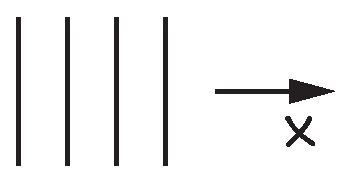
\includegraphics{1.eps} %ширина рисунка составляет половину от ширины текста, picture1 - название файла с изображением, помещенного в папку Images
	\caption{Волна по $ x $}
	\label{fig::1}
\end{figure}

Ищем однородное решение по $ x $ и $ z $
[ под однородностью понимается отсутствие зависимости от $ x $ и $ z $, её одинаковость ].

\begin{equation*}
\frac{\partial \vec{v}_{x}}{\partial t} + \frac{1}{\rho_{0}}\:\left( \frac{\partial p}{\partial \rho} \right)_{S} \frac{\partial\rho\:'}{\partial x} = 0.
\end{equation*}
про diff по времени и получим:
\begin{equation}\label{12}
\frac{\partial^{2} \vec{v}_{x}}{\partial t^{2}} + \frac{1}{\rho_{0}}\:\left( \frac{\partial p}{\partial \rho} \right)_{S} \frac{\partial}{\partial x}\frac{\partial\rho\:'}{\partial t} = 0.
\end{equation}

А теперь из второго выражения (\ref{10}) выразим $ \frac{\partial \rho \: '}{\partial t} $

\begin{equation}\label{13}
\frac{\partial \rho\:'}{\partial t} = - \rho_{0}\: div(\vec{v}) = - \rho_{0}\: \frac{\partial v_{x}}{\partial x}
\end{equation}

Подставим (\ref{13}) в (\ref{12}) и получим:


\begin{equation}\label{14}
\frac{\partial^{2} \vec{v}_{x}}{\partial t^{2}} - \frac{1}{\rho_{0}}\:\left( \frac{\partial p}{\partial \rho} \right)_{S} \frac{\partial}{\partial x}\:\rho_{0}\: \frac{\partial v_{x}}{\partial x} = 0.
\end{equation}

В результате имеем:
\begin{equation}\label{15}
\frac{\partial^{2} v_{x}}{\partial t^{2}} - \left( \frac{\partial p}{\partial \rho} \right)_{S}
\frac{\partial^{2} v_{x}}{\partial x^{2}} = 0
\end{equation}

Обозначим $ \left( \frac{\partial p}{\partial \rho} \right)_{S} = c^{2} $, вот и получилось уравнение плоской волны.

\begin{equation}\label{16}
\frac{\partial^{2} v_{x}}{\partial t^{2}} - c^{2}
\frac{\partial^{2} v_{x}}{\partial x^{2}} = 0
\end{equation}

Это гиперболическое уравнение мат.физики 
(существуют три вида:)
\begin{itemize}
	\item Параболического типа
	\item Эллиптического типа 
	\item  Гиперболического типа 
\end{itemize}

В итоге у нас есть равнение гиперболического типа с 1й неизвестной, но порядок повысился (квадраты и всё такое), уравнение второго порядка по времени и координате.

Получили волновое уравнение гиперболического типа, где
$ c $ - скорость волны, попрошу внимания "звуковой волны". Теперь решим это уравнение.
Решение в отличие от детского сада получим на более высоком уровне.

Так как движения описываемые уравнение Эйлера являются потенциальными.
Введём как в электродинамике потенциал. Введём потенциал скорости $ \vec{v} = \nabla \varphi $, где $ \varphi $ - потенциал скорости. Через потенциал скорости можно найти все интересующие нас величины.

Из уравнения Эйлера 
\begin{equation}\label{17}
\nabla\frac{\partial \varphi}{\partial t} = - \frac{1}{\rho_{0}}\nabla p\:' \Rightarrow p\:' \: = \: - \rho_{0} \frac{\partial \varphi}{\partial t}
\end{equation}

То есть если известно $ \varphi $ - то можно без проблем найти изменение давления колебаний.

Из уравнения состояния (\ref{8}) имеем $ p' = c^{2}  \rho\:' $  и можем выразить плотность $ \rho\:' $:
\begin{equation}\label{18}
\rho\:' = \frac{p\:'}{c^{2}} = - \frac{\rho_{0}}{c^{2}}\frac{\partial \varphi}{\partial t}.
\end{equation}

Вернёмся к уравнению непрерывности (неразрывности) (\ref{10}) используя $ p\:' $.
\begin{equation*}
\frac{\partial \rho\:'}{\partial t} + \rho_{0}\:\left( \frac{\partial p}{\partial \rho} \right)_{S} div(\vec{v}) = 0 \Rightarrow - \rho_{0}\:\frac{\partial^{2} \varphi}{\partial t^{2}} + \rho_{0}\left( \frac{\partial p}{\partial \rho} \right)_{S} div(grad(\varphi)) = 0
\end{equation*}

То есть снова пришли к волновому уравнению:
\begin{equation}\label{20}
\frac{\partial^{2} \varphi}{\partial t^{2}} - c^{2} \triangle \varphi = 0
\end{equation}

Вывод потенциал скорости тоже подчиняется волновому уравнению.
Найдём для начала решение одномерного уравнения (\ref{20}), для того чтобы его решить перейдём к переменным $ \xi = x - ct $ и $ \eta = x + ct $. Переработаем уравнение в терминах новых переменных 

\begin{equation}\label{21}
\frac{\partial \varphi}{\partial x} = \frac{\partial \varphi}{\partial \eta}\frac{\partial \eta}{\partial x} + \frac{\partial \varphi}{\partial \xi}\frac{\partial \xi}{\partial x} =  \frac{\partial \varphi}{\partial \eta}\cdot 1 + \frac{\partial \varphi}{\partial \xi}\cdot 1 = \frac{\partial \varphi}{\partial \eta} + \frac{\partial \varphi}{\partial \xi}
\end{equation}
 Используем это для получения второй производной:
 \begin{eqnarray*}
 \frac{\partial^{2} \varphi}{\partial x^{2}} = \frac{\partial}{\partial x} \left( \frac{\partial \varphi}{\partial \eta} + \frac{\partial \varphi}{\partial \xi} \right) = \frac{\partial }{\partial \eta}\frac{\partial \varphi}{\partial x} + \frac{\partial}{\partial \xi}\frac{\partial \varphi}{\partial x} \\
  = \frac{\partial }{\partial \eta} \left( \frac{\partial \varphi}{\partial \eta} + \frac{\partial \varphi}{\partial \xi} \right) + \frac{\partial }{\partial \xi} \left( \frac{\partial \varphi}{\partial \eta} + \frac{\partial \varphi}{\partial \xi} \right) = \\
   \frac{\partial^{2} \varphi}{\partial \eta^{2}} + \frac{\partial^{2} \varphi}{\partial \eta \partial \xi} + \frac{\partial^{2} \varphi}{\partial \xi \partial \eta} + \frac{\partial^{2} \varphi}{\partial \xi^{2}} = 
      \frac{\partial^{2} \varphi}{\partial \eta^{2}} + \frac{2\:\partial^{2} \varphi}{\partial \eta \partial \xi} +  \frac{\partial^{2} \varphi}{\partial \xi^{2}}
 \end{eqnarray*}
Подобным образом распишем производную по времени:
\begin{eqnarray}\label{23}
\frac{\partial \varphi}{\partial t} = \frac{\partial \varphi}{\partial \eta}\frac{\partial \eta}{\partial t} + \frac{\partial \varphi}{\partial \xi}\frac{\partial \xi}{\partial t} = \frac{\partial \varphi}{\partial \eta}\cdot c - \frac{\partial \varphi}{\partial \xi}\cdot c
\end{eqnarray}

 \begin{eqnarray*}
\frac{\partial^{2} \varphi}{\partial t^{2}} = \frac{\partial}{\partial t}\left[ c \cdot \left( \frac{\partial \varphi}{\partial \eta} - \frac{\partial \varphi}{\partial \xi} \right)\right]  = c \cdot \frac{\partial }{\partial \eta}\frac{\partial \varphi}{\partial t} - c\cdot \frac{\partial}{\partial \xi}\frac{\partial \varphi}{\partial t} \\
= c\cdot \frac{\partial }{\partial \eta} \left( \frac{\partial \varphi}{\partial \eta}\cdot c -  \frac{\partial \varphi}{\partial \xi}\cdot c \right) - c\cdot \frac{\partial }{\partial \xi} \left( \frac{\partial \varphi}{\partial \eta}\cdot c - \frac{\partial \varphi}{\partial \xi} \cdot c \right) = \\
c^{2}\cdot\frac{\partial^{2} \varphi}{\partial \eta^{2}} - c^{2}\cdot \frac{\partial^{2} \varphi}{\partial \eta \partial \xi} - c^{2}\cdot \frac{\partial^{2} \varphi}{\partial \xi \partial \eta} + c^{2}\cdot \frac{\partial^{2} \varphi}{\partial \xi^{2}} = 
c^{2}\cdot \left[ \frac{\partial^{2} \varphi}{\partial \eta^{2}} - \frac{2\:\partial^{2} \varphi}{\partial \eta \partial \xi} +  \frac{\partial^{2} \varphi}{\partial \xi^{2}}\right] 
\end{eqnarray*}

Теперь подставим в уравнение (\ref{20}), которое записывается в нашем случае следующим образом $ \frac{\partial^{2} \varphi}{\partial t^{2}} - c^{2} \frac{\partial^{2} \varphi}{\partial x^{2}} = 0 $

В итоге имеем следующее равенство:

\begin{equation}\label{25}
4c^{2}\cdot \frac{\partial^{2} \varphi}{\partial \eta \partial \xi} = 0 \Rightarrow \frac{\partial^{2} \varphi}{\partial \eta \partial \xi} = 0
\end{equation}
Уравнение (\ref{25}) легко решить.
Найдём общее решение этого уравнения.

После первого интегрирования по $ \eta $ получим:
\begin{equation*}
\frac{\partial \varphi}{\partial \xi} = f(\xi)
\end{equation*}
Второе интегрирование даёт:
\begin{equation*}
\varphi = \underbrace{\int f_{1}(\xi)d\xi}_{\text{переходит в}\tilde{f_{1}}(\xi)} + f_{2}(\eta)
\end{equation*}

Упустим тильду и получим следующее :
\begin{equation*}
\varphi = f_{1}(\xi) + f_{2}(\eta).
\end{equation*}
Это одно из фундаментальных свойств гиперболического уравнения.
Вернёмся к исходным переменным:
\begin{equation}\label{29}
\varphi = f_{1}(x-ct) + f_{2}(x+ct).
\end{equation}
И это говорит нам о том, что волна может иметь любую форму главное чтобы это решение зависело от волнового аргумента.
Волновой аргумент говорит о том что при смещении координаты $ x $ на $ ct $ значение волнового аргумента в следующий момент времени $ t $ не меняется это справедливо для каждой точки $ x $.
Эти два частных решения независимы и именно отсюда и видно, что $ c $ - скорость рассматриваемой волны.

Итак исходное волновое уравнение описывает без дисперсионную волну. Так как вся картина движется (перемещается) в среде со скоростью $ c $ без дисперсии.
 
"Дисперсия волн — в теории волн различие фазовых скоростей линейных волн в зависимости от их частоты. Дисперсия волн приводит к тому, что волновое возмущение произвольной негармонической формы претерпевает изменения (диспергирует) по мере его распространения."

Отметим тот факт, что звуковая волна в жидкостях и газах является продольной 
\begin{equation}\label{30}
\varphi(x,t) \: \Rightarrow \: v_{x}=\nabla_{x}\: \varphi = \frac{\partial \varphi}{\partial x}.
\end{equation}

Далее ограничимся одним частным решением, которое описывает волну в положительном направлении $ x $.

\begin{equation}\label{31}
 v_{x}=\nabla_{x}\: \varphi = \frac{\partial \varphi}{\partial x}= f\:'(x-ct) = \frac{\partial f}{\partial \xi} \cdot 1.
\end{equation}

Найдём давление $p\:'$:
\begin{equation}\label{32}
p\:' = - \rho_{0} \frac{\partial \varphi}{\partial t} =  - \rho_{0} \:f\:'(x-ct)\cdot(-c) = \rho_{0}\:c \:f\:'(x-ct)
\end{equation}
Исключим $ f' $ из уравнения (\ref{31})
\begin{equation*}
p\:' = \rho_{0}\:c \: v_{x} \Rightarrow  v_{x} = \frac{p\:'}{\rho_{0}\:c}
\end{equation*}
Если воспользоваться уравнением состояния записанного ранее (\ref{18}) $ p' = c^{2}  \rho\:' $ выражение для скорости приобретёт следующий вид:
\begin{equation*}
v_{x}= \frac{c \rho\:'}{\rho_{0}}.
\end{equation*}
По всему выходит, что все величины завязаны друг на друге.

Мини итог:
\begin{enumerate}
	\item Получили решение для двух волн $ f_{1} + f_{2} $.
	\item Получили связь.
\end{enumerate}

\newpage

\begin{center}
	\section*{Вторая пара 10.01.19} % Звездочка убирает нумерацию главы
	\addcontentsline{toc}{section}{Вторая пара 10.01.19} % Добавляет Введение в Содержание
\end{center}

При описании звуковой волны мы предполагали, что среда адиабатическая.
То есть для системы выполняется Закон Сохранения Энергии.
В уравнении Эйлера также нет вязкости, это не противоречит тому что в ходе распространения волны температура может изменятся.

Это подтверждает идею перехода энергии кинетической в потенциальную и обратно.

Обратимся к всемогущей термодинамике:
\begin{equation}\label{35}
p (\rho , S) = \left( \frac{\partial p}{\partial \rho}\right)_{S}  \rho\:' + \underbrace{\left( \frac{\partial p}{\partial S}\right)_{\rho}  S\:'}_{\text{даёт }\: 0 \: \text{т.к проц адиабатический }}
\end{equation}
по аналогии :

\begin{equation}\label{36}
T\:' = T\:' (\rho , S) = \left( \frac{\partial T}{\partial \rho}\right)_{S}  \rho\:' + \underbrace{\left( \frac{\partial T}{\partial S}\right)_{\rho}  S\:'}_{\text{даёт }\: 0 }.
\end{equation}
 то есть имеем такого рода формулу:
 \begin{equation}\label{37}
 T\:'= \left( \frac{\partial T}{\partial \rho}\right)_{S}  \rho\:'.
 \end{equation}
 Но это как бывает только для слабых отклонений.
 
Вспомним за коэффициент температурного расширения $ \frac{1}{V}\bracket{\frac{\partial V}{\partial T}}_{p} = \beta  $ 
Также поговорим за энтальпию:
"энтальпия определяется как сумма внутренней энергии $ \varepsilon $ и произведения давления $ P $ на объём $ V $"
 \begin{equation}\label{38}
H = \varepsilon + pV
\end{equation}
Из уравнения внутренней энергии известно, что :
\begin{equation}\label{39}
d\varepsilon = TdS - pdV
\end{equation}
То есть получаем:
\begin{equation}\label{40}
dH = d(\varepsilon) + d(pV) = TdS - pdV + pdV +Vdp = TdS + Vdp
\end{equation}
Отсюда вытекают следующие соотношения:
\begin{equation}\label{41}
 \bracket{\frac{\partial T}{\partial p}}_{S} = \bracket{\frac{\partial V}{\partial S}}_{p} = \bracket{\frac{\partial V}{\partial T}}_{p}\bracket{\frac{\partial T}{\partial S}}_{p} = \frac{T}{C_{p}}\bracket{\frac{\partial V}{\partial T}}_{p}
\end{equation}
\begin{equation}\label{42}
T\:' = \frac{T}{C_{p}}\beta V_{0}p\:' = \text{подставляем}\:\: p\:'=  \frac{T}{C_{p}}\beta V_{0}\frac{C}{V_{0}}v = \frac{T}{C_{p}}\beta v C 
\end{equation}
Выражение (\ref{42}) очень важно. 
Эти соотношение демонстрируют, что все величины в звуковой волне меняются синхронно.

Вот ещё 2 ТД тождества 
\begin{equation}\label{43}
\bracket{\frac{\partial p}{\partial \rho}}_{S} = \frac{C_{p}}{C_{v}}\bracket{\frac{\dd{p}}{\dd{\rho}}}_{T}
\end{equation}

\begin{equation}\label{43.1}
\bracket{\frac{\partial p}{\partial \rho}}_{S} = \frac{C_{p}}{C_{v}}\bracket{\frac{\dd{p}}{\dd{V}}}_{T}
\end{equation}

Докажем это чуть позже !!ПОЗЖЕ!!


Известно соотношение, что $ C_{p}\: > \: C_{v} $
Вспомним, что теплоёмкость это энергия которая необходима для того чтобы нагреть тело на $ 1 $ градус. 
\begin{equation*}
\underbrace{\bracket{\frac{\partial p}{\partial \rho}}_{S}}_{\text{Сжимаемость}} = \frac{C_{p}}{C_{v}}\bracket{\frac{\dd{p}}{\dd{\rho}}}_{T} = \text{Обозначим} = \gamma\bracket{\frac{\dd{p}}{\dd{\rho}}}_{T},
\end{equation*}
где $ \gamma $ - отношение теплоёмкостей.

Вот и оказывается что скорость $ c $:
\begin{equation*}
c^{2} = \underbrace{\bracket{\frac{\dd{p}}{\dd{\rho}}}_{S}}_{\text{Это нельзя выяснить теоретически}} = \gamma\bracket{\frac{\dd{p}}{\dd{\rho}}}_{T},
\end{equation*}
Воспользуемся уравнением состояния газа:
\begin{equation}\label{46}
\frac{pV}{T} = R\frac{m}{\mu},
\end{equation}
для элемента газа единица массы будем иметь:
\begin{equation}\label{47}
p = \rho\: T\frac{R}{\mu},
\end{equation} 
где $ R $ -газовая постоянная 
отсюда и возьмём производную.
\begin{equation}\label{48}
\bracket{\frac{\dd{p}}{\dd{\rho}}}_{T} = \frac{TR}{\mu},
\end{equation} 
можно к примеру выразить скорость звука.
\begin{equation*}
c^{2} = \gamma\bracket{\frac{\dd{p}}{\dd{\rho}}}_{T},
\end{equation*}
\begin{equation}\label{50}
c = \sqrt{\gamma\bracket{\frac{\dd{p}}{\dd{\rho}}}_{T}} = \sqrt{\gamma\bracket{\frac{TR}{\mu}}},
\end{equation}
 
Прикинем скорость звука при $ T = 300K, R = 8.31, \gamma = 1.4, \mu = 0.029$.
При таких значениях $ C = 347 \frac{\text{кг}}{\text{моль}}$

Но обычно делают наоборот используют скорость звука для определения показателя адиабаты - $ \gamma $  

Сжимаемость воздуха сильно зависит от сжатия.
\begin{equation*}
C = \sqrt{\gamma\bracket{\frac{\dd{p}}{\dd{\rho}}}_{T}} = \sqrt{\gamma\bracket{\frac{TR}{\mu}}},
\end{equation*}
это видно из формулы (\ref{50}) выше  (Формула Лапласа для скорости звука).
$ \gamma $ и $ \mu $ - материальные параметры
$ T $ - регулируемый параметр $ C \sim \sqrt{T} $.

\begin{equation}\label{51}
\frac{\dd{^{2}\:\varphi}}{\dd{t^{2}}} = C^{2}\Delta\:\varphi
\end{equation}

\underline{Монохроматические волны} - гармонические функции по времени. Будем искать решение этого уравнения в экспоненциальной форме.
$ \varphi(x,y,z,t) $.

\begin{equation*}
\varphi = Re\left\lbrace \varphi_{0}\e\right\rbrace 
\end{equation*}
P.S. - мы используем только реальную часть, потому что скорость не может быть мнимой.

Если ищем в таком виде то мы отделяем временную переменную .
$ \varphi_{0} $ - это не просто амплитуда, а амплитуда (x,y,z)
Мы отделяем временную переменную 
\begin{equation}\label{53}
\varphi = Re\left\lbrace \varphi_{0}\e\right\rbrace \Rightarrow \frac{\dd{^{2}\:\varphi}}{\dd{t^{2}}} = C^{2}\Delta\:\varphi
\end{equation}
\begin{equation*}
-\varphi_{0}\: \omega^{2}\e = C^{2}\:\Delta\: \varphi_{0}\e
\end{equation*}
преобразуем
\begin{equation*}
-\varphi_{0}\: \omega^{2} = C^{2}\:\Delta\: \varphi_{0}
\end{equation*}
\begin{equation*}
\Delta\: \varphi_{0} + \varphi_{0}\: \frac{\omega^{2}}{C^{2}} = 0 
\end{equation*}
Пусть будем рассматривать вновь только ось $ x $, получаем:
\begin{equation*}
\frac{\dd{^{2}\varphi_{0}}}{\dd{x^{2}}} + \varphi_{0}\: \frac{\omega^{2}}{C^{2}} = 0 
\end{equation*}
Ого себе получили уравнение гармонических колебаний.
\begin{equation*}
\varphi_{0}\: \sim e^{i\:\sqrt{\frac{\omega^{2}}{C^{2}}}x}\sim e^{i\:\frac{\omega}{C}x} 
\end{equation*}

Это мы подставляем и оставляем только одну часть распространения волны.
\begin{equation}\label{54}
\varphi =  Re\left\lbrace Ae^{i\bracket{\frac{\omega}{C}x - \omega t}} \right\rbrace = Re\left\lbrace Ae^{i\bracket{kx - \omega t}} \right\rbrace 
\end{equation}
Если ищем решения в виде монохроматической волны $ \omega $
$ A $ - отвечает за сдвиг фазы
$ k $ - волновое число, оно показывает пространственную периодичность волны и связан с длиной волны.
\begin{equation*}
k = \frac{2\pi}{\lambda}
\end{equation*}
\begin{equation*}
\frac{\omega}{c} = \frac{2\pi}{\lambda}
\end{equation*}
\begin{equation*}
\lambda = \frac{2\pi\: c}{\omega}
\end{equation*}
$ A $ так как комплексное число то запишем его как $ A = a\:e^{i\alpha} $
где $ a $ -амплитуда и тогда можно подставить в (\ref{54}) и досчитать.
\begin{equation*}
\varphi =  a\: \cos(kx-\omega t + \alpha)
\end{equation*}
Описывает волну движущая в направлении положительных $ x $.

Обобщая на 3х  мерный случай получим волновой вектор $ \vec{k}(k_{x},k_{y},k_{z}) $ от $ k_{x}x; k_{y}y; k_{z}z \Rightarrow \vec{k}\vec{r} $, переходим к скалярному произведению.

\begin{equation*}
\varphi =  Re\left\lbrace Ae^{i\bracket{\vec{k}\vec{r} - \omega t}} \right\rbrace 
\end{equation*}
волновой вектор нужно записать: $\:\: \vec{k} = k_{x}\vec{i} + k_{y}\vec{j} + k_{z}\vec{z} \:\: $ и $\:\: \vec{k} = |k|\:\vec{n} = \frac{\omega}{c}, $
где $ \vec{n} $ - вектор направленный перпендикулярно фронту волны (где движется волна).

В общем случае монохроматические волны можно разложить в любую самую сложную волну. - это важный вывод.

\newpage
\begin{center}
	\subsection*{Энергия и импульс звуковых волн} % Звездочка убирает нумерацию главы
	\addcontentsline{toc}{subsection}{Энергия и импульс звуковых волн} % Добавляет Введение в Содержание
\end{center}
Найдём для начала энергию заключённую волне (рис.\ref{fig::1}).

Энергия в единице объёма жидкости как мы знаем представлена следующим неравенством:
\begin{equation}\label{57}
\rho \: \varepsilon + \frac{\rho \: v^{2}}{2},
\end{equation}
 конечно, оно для идеальной жидкости, а $ \varepsilon $ -внутренняя энергия единицы объёма, приход на единицу объёма.
 
 Где первое слагаемое внутренняя энергия, а второе кинетическая энергия.
 Разложим 
\begin{equation*}
\rho = \rho_{0} +\rho\:'
\end{equation*}
\begin{equation*}
 \varepsilon =  \varepsilon_{0} + \varepsilon\:'
\end{equation*}
Как и ранее колебания не большие для плотности и энергии. К сожалению, скорость мы так разложить не можем так как волна покоится.
Разложим выражение  $ \rho\:\varepsilon $ на $ \rho $ и $ S $ то есть по ТД параметрам.

\begin{equation*}
 \rho\:\varepsilon =  \rho_{0}\:\varepsilon_{0} + \bracket{\frac{\dd{ (\rho\:\varepsilon) }}{\dd{\rho}}}_{S} \: \rho\:' + \frac{1}{2}\bracket{\frac{\dd{^{2} (\rho\:\varepsilon) }}{\dd{\rho\:^{2}}}}_{S} \: \rho\:'\:^{2} + ...
\end{equation*}
Отсутствие слагаемых с $ S $ - связано с тем что процесс адиабатический.
Из первого начала тд известно что $ d\varepsilon = TdS - pdV = TdS - \frac{p}{\rho\:^{2}}d\rho$, а $ H = \varepsilon + \frac{p}{\rho}$.
\begin{equation*}
 dH = d\varepsilon + \frac{p}{\rho} + \frac{p}{\rho\:^{2}}d\rho = TdS + \frac{p}{\rho\:^{2}}d\rho + \frac{p}{\rho} + \frac{p}{\rho\:^{2}}d\rho =  TdS + \frac{p}{\rho} 
\end{equation*}
Всё это необходимо для работы с производными в разложении.
\begin{equation*}
\bracket{\frac{\dd{\varepsilon}}{\dd{\rho}}}_{S} = \frac{p}{\rho\:^{2}}
\end{equation*}
\begin{equation*}
\bracket{\frac{\dd{H}}{\dd{p}}}_{S} = \frac{1}{\rho}
\end{equation*}
Поработаем с производной:
\begin{equation*}
 \bracket{\frac{\dd{ (\rho\:\varepsilon) }}{\dd{\rho}}}_{S} = \varepsilon + \rho\:\bracket{\frac{\dd{\varepsilon}}{\dd{\rho}}}_{S} = \varepsilon +  \frac{p}{\rho} = \varepsilon + pV = H
\end{equation*}
Неожиданно получили энтальпию.

\begin{equation*}
\dif{H}{\rho}_{S} = \dif{H}{p}_{S}\dif{p}{\rho}_{S} = \frac{1}{\rho}c^{2}
\end{equation*}

\begin{equation}\label{59}
\rho\:\varepsilon = \rho_{0}\:\varepsilon_{0} + H_{0}\rho\:' + \frac{1}{2}\frac{c^{2}}{\rho_{0}}\rho\:'\:^{2} +...
\end{equation}

Разберём наше разложение (\ref{59}):
Первое слагаемое $ H_{0}\rho\:' $ - это энергия единицы объёма неподвижной жидкости в которой отсутствуют колебания. Его мы отбрасываем потому что нас интересуют именно звуковые колебания.
Второе слагаемое $ H_{0}\rho\:' $  - изменение энергии элемента жидкости связанного с его массой. Его мы отбрасываем по причине $ \int \rho\:' dV = 0 $ так как в звуковой волне среднее значение $ \bar{\rho}\:' = 0 $.
Остаётся слагаемое $ \frac{1}{2}\frac{c^{2}}{\rho_{0}}\rho\:'\:^{2} $ говоря человеческим языком деформация энергии.

В результате полная энергия определяется 
\begin{equation*}
\int_{V}\bracket{\frac{\rho_{0} \: v^{2}}{2} + \frac{c^{2}\:\rho\:'\:^{2}}{2\:\rho_{0}}}dV
\end{equation*}

Теперь запишем энергию единицы объёма звуковой волны:
\begin{equation}\label{61}
E = \frac{\rho_{0} \: v^{2}}{2} + \frac{c^{2}\:\rho\:'\:^{2}}{2\:\rho_{0}}
\end{equation}
и она, оказывается аналогичной энергии пружины.

Если же вернуться к энергии плоской звуковой волны справедливо, что $ v = \frac{c\:\rho\:'}{\rho_{0}} $ можно выразить $ \:\rho\:' $ и подставить в (\ref{61}):
\begin{equation}\label{62}
E = \frac{\rho_{0} \: v^{2}}{2} + \frac{c^{2}\:\rho_{0}^{2}\:v^{2}}{2\:\rho_{0}} = \rho_{0}\:v^{2}
\end{equation}
Вот так мы получили выражение (\ref{62}) для плотности энергии звуковой волны.
И это, оказывается характерным для любого гармонического осциллятора. Ну и ,конечно,звуковая волна обладает определённой энергией.
\newpage
\begin{center}
	\section*{Третья пара 16.01.19} % Звездочка убирает нумерацию главы
	\addcontentsline{toc}{section}{Третья пара 16.01.19} % Добавляет Введение в Содержание
\end{center}
Плотность энергии связана с кинетической энергией и деформацией.
$ E $ - это энергия при осреднении по времени даёт не нулевое значение.
Найдём плотность потока энергии звуковой волны. 

Плотность потока энергии - это количество энергии проходящее через единицу площади за единицу времени.
В гидродинамике она представляет собой 
\begin{equation*}
\rho \vec{v} \bracket{\frac{v^{2}}{2} + H}
\end{equation*}
Если от него взять $ div $, то мы получим:
\begin{equation*}
\rho \varepsilon + \frac{\rho\:v^{2}}{2} 
\end{equation*}
Но сейчас нас интересует доля от плотности потока энергии связанная с звуковой волной.
Раскладывая $ \rho \vec{v} \bracket{\frac{v^{2}}{2} + H} $ заметим, что $  \rho \vec{v}H \gg \frac{\rho\:v^{2}}{2}\vec{v} $. Далее мы разложим все интересующие нас величины в ряд.
\begin{equation*}
H = H_{0} + H'
\end{equation*}
\begin{equation*}
H\:' = \dif{H}{p}_{S}p\:'
\end{equation*}
Одно слагаемое обусловлено как и раньше адиабатичностью процесса. И подставляя это получаем следующее выражение:
\begin{equation*}
 \rho\:\vec{v}H = \rho\:\vec{v}H_{0} + \rho\:\vec{v}H\:' = \rho\:\vec{v}H_{0} + \rho\:\frac{p\:'\vec{v}}{\rho}
\end{equation*}
В итоге полный поток энергии за единицу времени будет равняться следующему соотношению:
\begin{equation*}
\oint \bracket{ \rho\:\vec{v}H_{0} + p\:'\vec{v}}d \vec{S}
\end{equation*}
Отбрасываем слагаемое $ \rho\:\vec{v}H_{0} $, потому что этот поток энергии связан с изменением массы.
Таким  образом плотность потока энергии обусловленная звуковой волна равна:
\begin{equation}\label{63}
\vec{q} = p\:'\vec{v}
\end{equation}
Ну а полный поток равен 
\begin{equation*}
\oint p\:'\vec{v} d \vec{S}
\end{equation*}
Она получилась простой, потому что является продольной.

Легко доказать, что 
\begin{equation*}
\dif{E}{t} + div(p\:'\vec{v}) = 0 
\end{equation*}
ЭТО ДОМАШКА НА БАЛЛЫ тут тип теор Остроградского Гаусса пригодится ну и $ v = \frac{c}{\rho_{0}}\rho\:' $ рассматривать как в Ландавшице том гидродинамика.

Это соотношение выражает Закон сохранения Энергии применительно к звуковым колебаниям.
то есть связь:
\begin{equation*}
p\:' = vc \rho\: \Rightarrow \vec{q} = c v^{2} \rho \vec{n},
\end{equation*}
где $ \vec{n} $ - направлен по распространению волны колебаний. В итоге имеем схожую с электродинамикой формулу:
\begin{equation*}
\vec{q} = E c \vec{n},
\end{equation*}
где $ E $ объёмная плотность энергии.
В итоге в единице $ V $ заключена энергия и она переносится вдоль направления $ \vec{n} $ - единичного вектора, прошу заметить  со скорость $ c $.






\subsubsection*{Импульс звуковых волн} % Звездочка убирает нумерацию главы
\addcontentsline{toc}{subsubsection}{Импульс звуковых волн} % Добавляет Введение в Содержание
\begin{equation*}
\vec{j} = \vec{v}\rho ,
\end{equation*}
где $ \vec{j} $ - объёмная плотность вещества, или по-другому количество вещества проходящее через единицу площади, поток массы импульса единицы объёма.

В звуковой волне:
\begin{equation*}
\rho  = \rho_{0} + \rho\:',
\end{equation*}
где $ \rho\:' $ - отклонение плотности от некоторого среднего значения.

Подставим это в $ \vec{j} $:
\begin{equation*}
\vec{j} = \vec{v}\rho_{0}  + \vec{v}\rho \:' = \vec{v}\rho_{0} + \frac{p\:'}{c^{2}}\vec{v} = \vec{v}\rho_{0} + \frac{\vec{q}}{c^{2}}
\end{equation*}
Слагаемое $ \vec{v}\rho_{0} $ отбрасываем, потому что это энергия связанная с движением среды как целого.


Рассмотрим звуковую волну занимающую ограниченную площадь в пространстве (рис.\ref{fig::2}). Пусть движение потенциально то есть $ v = \nabla\varphi $/

\begin{figure}[h!] 	% Окружение для вставки иллюстрации
	\centering 		% Выравнивание по центру
	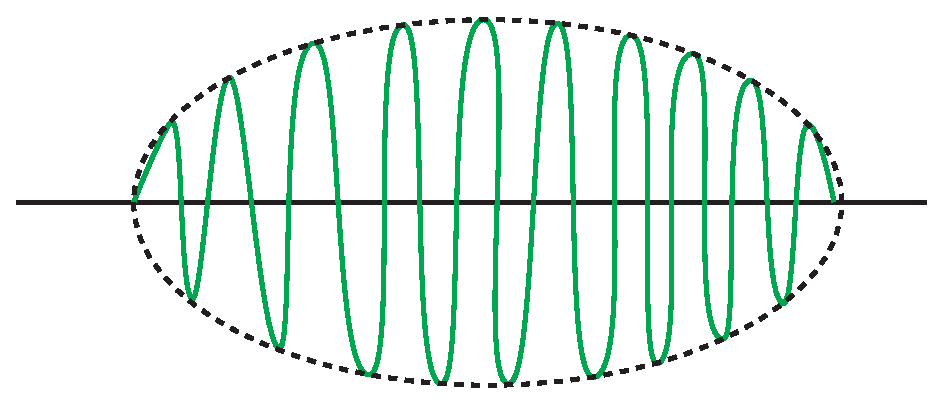
\includegraphics[width=12cm]{2.eps} %ширина рисунка составляет половину от ширины текста, picture1 - название файла с изображением, помещенного в папку Images
	\caption{Локализованная волна}
	\label{fig::2}
\end{figure}


Найдём полный импульс:
\begin{equation*}
\int \nabla\varphi \rho_{0}\:dV + \int \frac{\vec{q}}{c^{2}}\:dV
\end{equation*}
По теореме Остроградского-Гаусса имеем:
\begin{equation*}
\int \nabla\varphi\:dV = \oint \varphi \:d \vec{S}=0 
\end{equation*}
Ноль потому что $ \varphi_{\infty} = 0 $, то есть функция локализована в определённой области пространства, а это в свою очередь говорит о том, что среда как целое отброшена.
Тогда имеем: 
\begin{equation*}
\int \frac{\vec{q}}{c^{2}}\:dV
\end{equation*}
это и есть полный импульс по объёму.
Во втором порядке малости полный импульс переносимой волны не равен нулю.
Это означает, что имеет место отличный от нуля перенос вещества. Иными словами распространение звука сопровождается переносом вещества. Однако это перенос представляет собой эффект второго порядка малости.

\newpage
\begin{center}
	\subsection*{Отражение и преломление звуковых волн} % Звездочка убирает нумерацию главы
	\addcontentsline{toc}{subsection}{Отражение и преломление звуковых волн} % Добавляет Введение в Содержание
\end{center}
 Будем интересоваться откликом среды на взаимодействие звуковой волны с некоторой границей раздела (рис.\ref{fig::3}).
 
 Рассмотрим несколько возможных вариантов:
 \begin{enumerate}
 	\item Волна полностью отражается.
 	\item Волна частично, или полностью поглощается.
 \end{enumerate}

\begin{figure}[h!] 	% Окружение для вставки иллюстрации
	\centering 		% Выравнивание по центру
	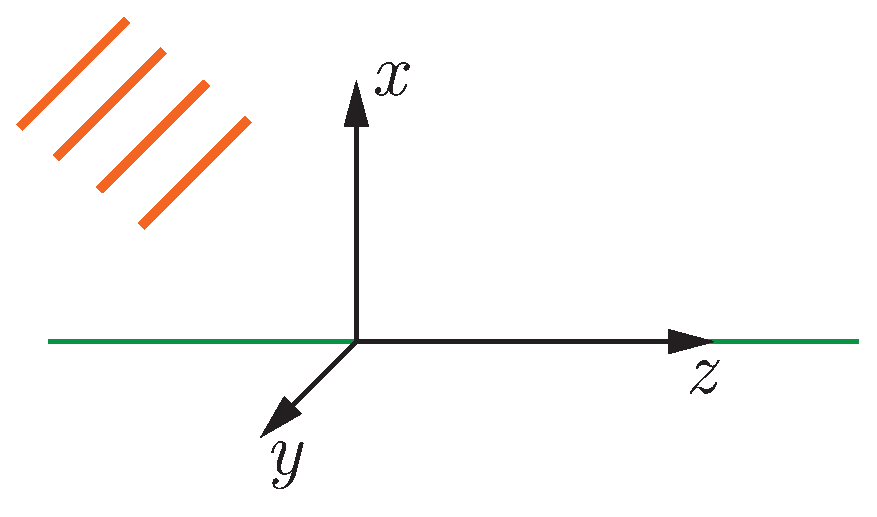
\includegraphics[width=12cm]{3.eps} %ширина рисунка составляет половину от ширины текста, picture1 - название файла с изображением, помещенного в папку Images
	\caption{Падающая волна}
	\label{fig::3}
\end{figure}

При падении звуковой волны на границу раздела двух различных сред в общем случае волна отражается и преломляется.
Так как рассматриваем сплошную среду  то логично что частоты волны сохраняются.
\begin{equation*}
\boxed{\omega_{1} = \omega_{2}} 
\end{equation*}

Случай первый: \underline{Отражение}

Главной особенность при отражении заключается в том, что движение в первой среде является результатом наложения двух волн падающей и отражённой.

Скорость звука падающей и отражённой волны должна быть одинакова, ибо всё происходит в одной среде.
\begin{equation*}
k_{1y} =k_{2y} 
\end{equation*}
\begin{equation*}
k_{1z} =k_{2z} 
\end{equation*}
 Волновые числа падающей ($ k_{1} $) и отражённой ($ k_{2} $) волны должны быть равны. $ z $ - компонента определяет периодичность по $ z $, а $ y $ по  $ y $.
 Стоит также учесть тот факт, что волновой вектор перпендикулярен фронту распространения волны.

\begin{figure}[h!] 	% Окружение для вставки иллюстрации
	\centering 		% Выравнивание по центру
	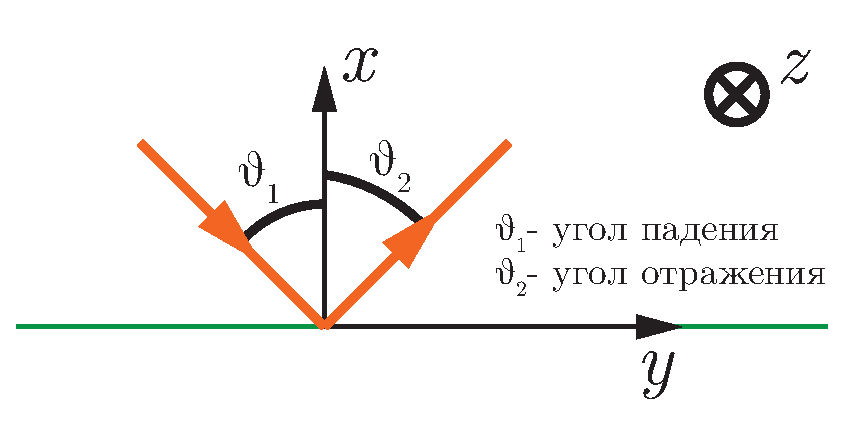
\includegraphics[width=12cm]{4.eps} %ширина рисунка составляет половину от ширины текста, picture1 - название файла с изображением, помещенного в папку Images
	\caption{Отражение}
	\label{fig::4}
\end{figure}

\begin{equation*}
k_{1y} = \frac{\omega}{c}\: sin(\: \vartheta_{1}\:) =  |k|\: sin(\: \vartheta_{1}\:)
\end{equation*}
\begin{equation*}
k_{2y} = \frac{\omega}{c}\: sin(\: \vartheta_{2}\:) =  |k|\: sin(\: \vartheta_{2}\:)
\end{equation*}
Равенство выше глаголит, что: \textit{"Угол падения равен углу отражения"}
\begin{equation*}
\: \vartheta_{1}\: =  \: \vartheta_{2}\:
\end{equation*}

Случай второй: \underline{Преломление звуковых волн}
\begin{figure}[h!] 	% Окружение для вставки иллюстрации
	\centering 		% Выравнивание по центру
	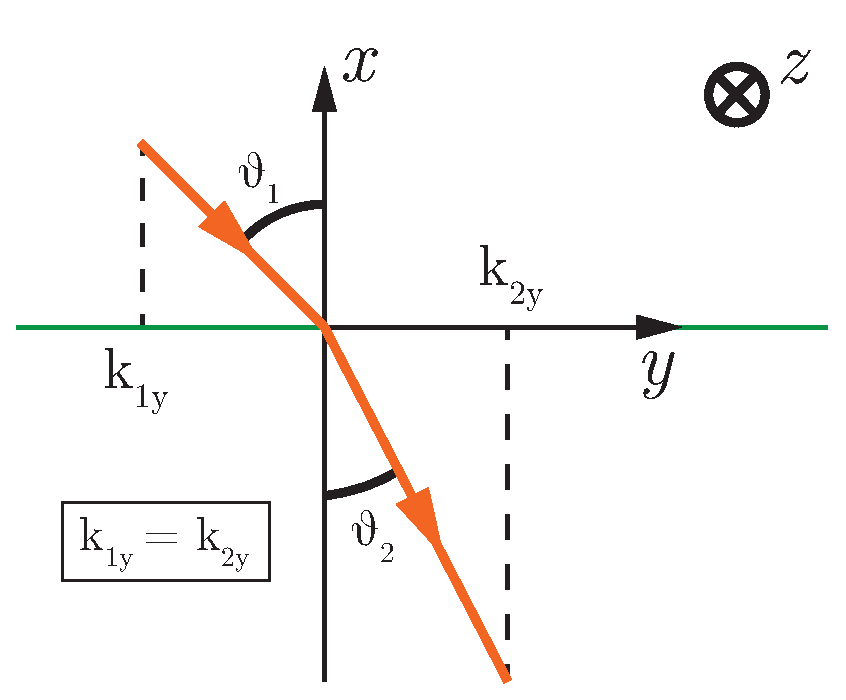
\includegraphics[width=12cm]{5.eps} %ширина рисунка составляет половину от ширины текста, picture1 - название файла с изображением, помещенного в папку Images
	\caption{Преломление}
	\label{fig::5}
\end{figure}

\begin{equation*}
k_{1y} = \frac{\omega}{c_{1}}\: sin(\: \vartheta_{1}\:) =  |k|\: sin(\: \vartheta_{1}\:)
\end{equation*}
\begin{equation*}
k_{2y} = \frac{\omega}{c_{2}}\: sin(\: \vartheta_{2}\:) =  |k|\: sin(\: \vartheta_{2}\:)
\end{equation*}
Но $ k_{1y} = k_{2y} $ меняется лишь $ x $  (рис.\ref{fig::5}). Поэтому приравнивая получаем:
\begin{equation*}
\frac{\omega}{c_{1}}\: sin(\: \vartheta_{1}\:) = \frac{\omega}{c_{2}}\: sin(\: \vartheta_{2}\:),
\end{equation*} 
Или по другому:
\begin{equation}\label{64}
\frac{sin(\: \vartheta_{1}\:)}{sin(\: \vartheta_{2}\:)}\:  = \frac{c_{1}}{c_{2}}\: ,
\end{equation}  
Вот и закон преломления.


\subsubsection*{Количественное соотношение между интенсивностями падающей, отражённой, преломлённой волны.} % Звездочка убирает нумерацию главы
\addcontentsline{toc}{subsubsection}{Количественное соотношение между интенсивностями падающей, отражённой, преломлённой волны.} % Добавляет Введение в Содержание
Найдём количественное соотношение между интенсивностями падающей, отражённой, преломлённой волны.  
Ограничимся 2х мерным пространством:
\begin{equation*}
\vec{k}\vec{r} = k_{x}x +k_{y}y \Rightarrow k  =\frac{\omega}{c},
\end{equation*} 
где $ k $ - величина волнового вектора.

Будем рассуждать в терминах потенциалов скорости:
\begin{equation*}
\varphi_{1} = A_{1}\: exp\left\lbrace i\omega\bracket{\frac{x}{c_{1}}\:cos(\:\vartheta_{1}\:) + \frac{y}{c_{1}}\:cos(\:\vartheta_{1}\:) -t} \right\rbrace  
\end{equation*} 
\begin{equation*}
\varphi_{1}' = A_{1}'\: exp\left\lbrace i\omega\bracket{-\frac{x}{c_{1}}\:cos(\:\vartheta_{1}\:) + \frac{y}{c_{1}}\:cos(\:\vartheta_{1}\:) -t} \right\rbrace  
\end{equation*} 
\begin{equation*}
\varphi_{2} = A_{2}\: exp\left\lbrace i\omega\bracket{\frac{x}{c_{2}}\:cos(\:\vartheta_{2}\:) + \frac{y}{c_{2}}\:cos(\:\vartheta_{2}\:) -t} \right\rbrace  
\end{equation*} 
$ \varphi_{1} $ - потенциал падающей волны, $ \varphi_{1}' $ - отражённой, $ \varphi_{2} $ - прошедшей.
Стоит упомянуть о:
\begin{equation*}
k = \frac{\omega}{c} \Rightarrow \omega (\:\frac{k}{\omega}\:x - t) \Rightarrow (kx - \omega t)
\end{equation*} 

Гран условия которые применяем таковы:
На поверхности раздела одинаковое давление.
\begin{equation*}
p = -\dot{\varphi}\rho = -\dif{\varphi}{t}\rho
\end{equation*} 
Его мы записываем и на потенциалы.
\begin{equation*}
v_{x} = \dif{\varphi}{x}
\end{equation*} 
На границе $ p_{1} = p_{2} $ и $ v_{x1} = v_{x2} $, а $ \dif{\varphi}\rho_{1} = \dif{\varphi}\rho_{2} $
В итоге получаем:
\begin{equation*}
 \begin{cases}
\rho_{1}\bracket{A_{1}-A_{1}'} = \rho_{1} A_{2} \\
\dif{\varphi_{1}}{x} = \dif{\varphi_{2}}{x}
\end{cases}
\end{equation*} 
И это всё при $ x = 0 $.
\begin{equation*}
\frac{cos(\:\vartheta_{1}\:)}{c_{1}}\bracket{A_{1}-A_{1}'}= \frac{cos(\:\vartheta_{2}\:)}{c_{2}}A_{2}
\end{equation*}

\newpage

\begin{center}
	\section*{Четвёртая пара 23.01.19} % Звездочка убирает нумерацию главы
	\addcontentsline{toc}{section}{Четвёртая пара 23.01.19} % Добавляет Введение в Содержание
\end{center}

Нормальная компонента скорости должна быть непрерывна - это относится к граничным условиям описанных выше.

\begin{equation*}
\begin{cases}
\rho_{1}\bracket{A_{1}-A_{1}'} = \rho_{1} A_{2} \\
\frac{cos(\:\vartheta_{1}\:)}{c_{1}}\bracket{A_{1}-A_{1}'}= \frac{cos(\:\vartheta_{2}\:)}{c_{2}}A_{2}
\end{cases}
\end{equation*} 

Определим коэффициент отражения:
$ R $ - представляет собой отношения средних по времени значений плотности потока энергий отражённой и падающей волны.
Это своеобразная доля отражённой энергии. 

\begin{figure}[h!] 	% Окружение для вставки иллюстрации
	\centering 		% Выравнивание по центру
	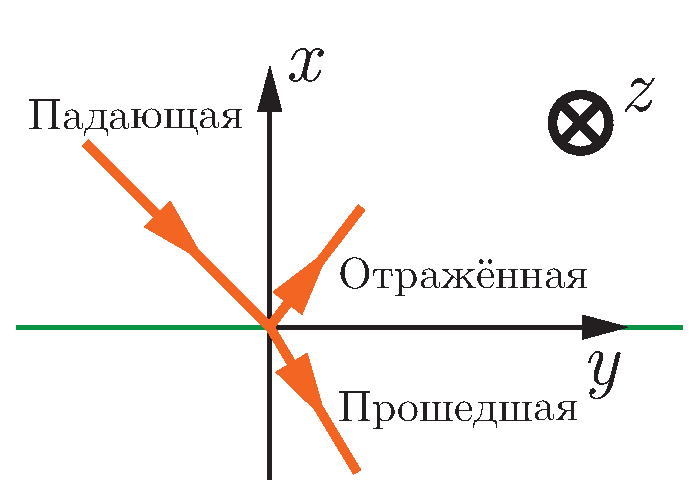
\includegraphics[width=12cm]{6.eps} %ширина рисунка составляет половину от ширины текста, picture1 - название файла с изображением, помещенного в папку Images
	\label{fig::6}
\end{figure}
Нужно помнить, что интенсивность падающей волны больше интенсивности отражённой волны, то же и для прошедшей (\ref{fig::6}).
Коэффициент прохождения будем обозначать $ D $ и это будет отношение прошедшей волны к падающей.

Как дз найти коэффициент прошедшей волны.

Сейчас же найдём коэффициент отражения $ R $, для этого воспользуемся вектором потока энергии (\ref{63})
\begin{equation*}
\vec{q} = cv^{2}\vec{n}\rho,
\end{equation*}
где $ \rho = \rho_{0} $, а $ v $ - связанно с колебаниями.
В итоге для $ R $ имеем:
\begin{equation*}
R = \frac{c_{1}\rho_{1}\:\overline{(v_{1}')^{2}}}{c_{1}\rho_{1}\:\overline{(v_{1})^{2}}} = \frac{|A_{1}'|^{2}}{|A_{1}|^{2}}
\end{equation*}
Так как $ v $ квадрат гармонической функции, то осреднение производится по времени и от экспоненты остаётся по $ \frac{1}{2} $ и они сокращаются в результате имеем только амплитуды.
$ A $-шки являются комплексными числами, потому что скорость вещества является величиной вещественной (какое-либо число), а вещественное число можно получить от произведения $ 2 $-х комплексных чисел. 

Из граничного условий получаем:
\begin{equation*}
\begin{cases}
\bracket{A_{1}-A_{1}'} = \frac{\rho_{1}}{\rho_{1}} A_{2} \\
\bracket{A_{1}-A_{1}'}= \frac{c_{1}}{c_{2}}\frac{\cos(\:\vartheta_{2}\:)}{\cos(\:\vartheta_{1}\:)}A_{2} 
\end{cases}
\end{equation*} 
Произведём замену по закону преломления (Снелла в оптике) (\ref{64}) $ \frac{sin(\: \vartheta_{1}\:)}{sin(\: \vartheta_{2}\:)}\:  = \frac{c_{1}}{c_{2}}\:  $, для второго выражения получим  
\begin{equation*}
\bracket{A_{1}-A_{1}'}= \frac{c_{1}}{c_{2}}\frac{\cos(\:\vartheta_{2}\:)}{\cos(\:\vartheta_{1}\:)}A_{2} = \frac{\sin(\: \vartheta_{1}\:)}{\sin(\: \vartheta_{2}\:)}\:\frac{\cos(\:\vartheta_{2}\:)}{\cos(\:\vartheta_{1}\:)}A_{2} = \frac{tg(\:\vartheta_{1}\:)}{tg(\:\vartheta_{2}\:)}A_{2}
\end{equation*}
Но тут $ 3 $ неизвестных амплитуды, а уравнений $ 2 $. Но это не страшно потому что нас интересуют не сами амплитуды, а их соотношения.
Выразим $ A_{1} $ и $ A_{1}' $, а потом сократим на $ A_{2} $
получим:
\begin{equation*}
2A_{1} = \frac{\rho_{2}}{\rho_{1}}  A_{2} + \frac{tg(\:\vartheta_{1}\:)}{tg(\:\vartheta_{2}\:)}A_{2}
\end{equation*}
\begin{equation*}
2A_{1}' = \frac{\rho_{2}}{\rho_{1}}  A_{2} - \frac{tg(\:\vartheta_{1}\:)}{tg(\:\vartheta_{2}\:)}A_{2}
\end{equation*}

А теперь найдём соотношение $ R $:
\begin{equation*}
R = \bracket{\frac{\frac{\rho_{2}}{\rho_{1}} - \frac{tg(\:\vartheta_{1}\:)}{tg(\:\vartheta_{2}\:)}}{ \frac{\rho_{2}}{\rho_{1}} + \frac{tg(\:\vartheta_{1}\:)}{tg(\:\vartheta_{2}\:)}}}^{2} = \bracket{\frac{\rho_{2}\:tg(\:\vartheta_{2}\:) - \rho_{1}\:tg(\:\vartheta_{1}\:)}{\rho_{2}\:tg(\:\vartheta_{2}\:) + \rho_{1}\:tg(\:\vartheta_{1}\:)}}^{2}
\end{equation*}
Видно, что данное выражение больше или равно нулю и меньше или равно единице.
Таким образом коэффициент отражения зависит от отношения плотностей и углов $ \vartheta_{1} $ и $ \vartheta_{2} $.

Интересным является рассмотрение коэффициента отражения $ R $, когда угол падения  $ \vartheta_{1} = 0 $.
Ибо тогда мы получаем неопределённость $ \frac{0}{0} $ используя закон отражения:
\begin{equation*}
\sin(\: \vartheta_{2}\:) = \frac{c_{2}}{c_{1}}\:\sin(\: \vartheta_{1}\:)
\end{equation*}
\begin{equation*}
\cos(\: \vartheta_{2}\:) = \sqrt{\bracket{1 - \sin^{2}(\: \vartheta_{2}\:) }} = \sqrt{\bracket{1 - \frac{c_{2}^{2}}{c_{1}^{2}}\:\sin^{2}(\: \vartheta_{1}\:) }}
\end{equation*}
И тогда получается:
\begin{equation*}
R = \bracket{\frac{\frac{\rho_{2}\:\frac{c_{2}}{c_{1}}\:\sin(\: \vartheta_{1}\:)}{\sqrt{\bracket{1 - \frac{c_{2}^{2}}{c_{1}^{2}}\:\sin^{2}(\: \vartheta_{1}\:) }}} - \rho_{1}\:\frac{\sin(\:\vartheta_{1}\:)}{\cos(\:\vartheta_{1}\:)}}{\frac{\rho_{2}\:\frac{c_{2}}{c_{1}}\:\sin(\: \vartheta_{1}\:)}{\sqrt{\bracket{1 - \frac{c_{2}^{2}}{c_{1}^{2}}\:\sin^{2}(\: \vartheta_{1}\:) }}} - \rho_{1}\:\frac{\sin(\:\vartheta_{1}\:)}{\cos(\:\vartheta_{1}\:)}}}^{2} = \bracket{\frac{\rho_{2}\:\frac{c_{2}}{c_{1}}\:\sin(\: \vartheta_{1}\:)\cos(\: \vartheta_{1}\:) - \rho_{1}\:\sin(\: \vartheta_{1}\:)\sqrt{...}}{\rho_{2}\:\frac{c_{2}}{c_{1}}\:\sin(\: \vartheta_{1}\:)\cos(\: \vartheta_{1}\:) + \rho_{1}\:\sin(\: \vartheta_{1}\:)\sqrt{...}}}^{2}
\end{equation*}
После преобразования, получаем:
\begin{equation*}
R = \bracket{\frac{\rho_{2}\:\frac{c_{2}}{c_{1}}\:\cos(\: \vartheta_{1}\:) - \rho_{1}\:\sqrt{...}}{\rho_{2}\:\frac{c_{2}}{c_{1}}\:\cos(\: \vartheta_{1}\:) + \rho_{1}\:\sqrt{...}}}^{2}  =\bracket{\frac{\rho_{2}\:c_{2}\cos(\:\vartheta_{1}\:) - \rho_{1}\:\sqrt{c^{2}_{1}-c^{2}_{1}\sin^{2}(\: \vartheta_{1}\:) }}{\rho_{2}\:c_{2}\cos(\:\vartheta_{1}\:) + \rho_{1}\:\sqrt{c^{2}_{1}-c^{2}_{1}\sin^{2}(\: \vartheta_{1}\:) }}}^{2} 
\end{equation*}
В пределе при $ \vartheta_{1} = 0 $ выходит:
\begin{equation*}
R =\bracket{\frac{\rho_{2}\:c_{2} - \rho_{1}\:c_{1}}{\rho_{2}\:c_{2} + \rho_{1}\:c_{1}}}^{2} 
\end{equation*}
\newpage
\begin{center}
	\subsection*{Геометрическая акустика} % Звездочка убирает нумерацию главы
	\addcontentsline{toc}{subsection}{Геометрическая акустика} % Добавляет Введение в Содержание
\end{center}

Звук - волна, амплитуда и направление распространения плоской волны неизменны во всём пространстве.
Направление определяется волновым вектором.
В случае произвольной звуковой волны её можно рассмотреть как плоскую на малом участке.
Для того чтобы это использовать необходимо на расстояния порядка длины звуковой волны неизменность направления и амплитуды.
Это позволяет использовать геометрическую акустику.

Луч - это линия, касательные к которой в каждой точке совпадают с направлением волны.
Геометрическая акустика отвечает пределу $ \lambda\longrightarrow0 $ 

Уравнение лучей - это основное уравнение геометрической акустики.
Оно даёт стационарную картину интенсивности звука.

Рассмотрим звуковые колебания без учёта диссипации. То есть движение элементов потенциально и это позволяет использовать потенциал скорости.

Мы хотим рассмотреть произвольную волну, для этого берём малую частичку и представляем в виде плоской.
И тогда потенциал в общем виде должен быть представлен как:
\begin{equation*}
\varphi = a \:e^{i\psi},
\end{equation*}
где $ a $ - это теперь медленно меняющаяся функция координат  и времени (меняется интенсивность звука). А $ \psi = \vec{k}\vec{r} - \omega t + \alpha $ - функция координаты и времени. $ \vec{k}\vec{r} - \omega t $ - аргументы в плоской волне, $ \alpha $ - некая фаза, $ \omega $ - циклическая частота.

Если разложить в ряд: 
\begin{equation*}
\psi = \psi_{0} + \vec{r}\:grad(\psi)+\dif{\psi}{t}t
\end{equation*}
Так как волна должна быть плоской получается, что отождествляя с выражением для плоской волны:
\begin{equation*}
grad(\psi) = \vec{k} \;\;\; \omega = -\dif{\psi}{t}
\end{equation*}
$ \psi $ - несёт в себе информацию о звуковой волне её называют \textbf{Эйконал}.
Эйконал с греческого изображение.

В звуковой волне имеем следующую связь:
\begin{equation*}
\frac{\omega^{2}}{c^{2}} = k^{2} =  k_{x}^{2} + k_{y}^{2} + k_{z}^{2}
\end{equation*}
Локально это свойство должно выполнятся.
В результате для уравнения Эйконала записывается в следующем виде:
\begin{equation*}
\dif{\psi}{x} + \dif{\psi}{y} + \dif{\psi}{z} - \frac{1}{c^{2}}\dif{\psi}{t} = 0
\end{equation*}
$ c^{2} $ - $  ( $ скорость звука $ )^{2} $ и также она функция координат если среда не однородна.

То есть Эйконал подчиняется нелинейному уравнению первого порядка с переменным коэффициентом.
Решение этого уравнения находится аналитически только в самых простейших случаях.

Аналогом действия  $ S $ и является Эйконал $ \psi $.
В механике действие - это скалярная функция, которая содержит в себе полную информацию ло состоянии системы в каждый момент времени. Если действие известно, то 
\begin{equation*}
\vec{p} = \dif{S}{\vec{r}}
\end{equation*}
Даёт импульс. 
\begin{equation*}
H = -\dif{S}{t}
\end{equation*}
Даёт функцию Гамильтона.
В геометрической акустике:
\begin{equation*}
\vec{k} = \dif{\psi}{\vec{r}}
\end{equation*}
\begin{equation*}
\omega = -\dif{\psi}{t}
\end{equation*}
Если мы отождествляем с механикой, тогда очевидно, что Эйконал является прямым аналогом действия.

Запишем уравнения Гамильтона:
\begin{equation*}
\dot{\vec{p}} = \dif{H}{\vec{r}}
\end{equation*}
Обобщённый импульс.
\begin{equation*}
\dot{\vec{r}} = -\dif{H}{p}
\end{equation*}
Заметим что $ \omega $ представляет собой аналог $ H $, а $ \vec{p} $ аналог $ \vec{k} $, тогда уравнения описывающие характеристику луча приобретут следующий вид:
\begin{equation*}
-\dot{\vec{k}} = \dif{\omega}{\vec{r}}
\end{equation*}
\begin{equation*}
\dot{\vec{r}} = \dif{\omega}{\vec{k}}
\end{equation*}
$ \dot{\vec{r}} $ координата луча по времени. По физическому смыслу $ \dot{\vec{r}} = с\vec{n} $, $ \vec{n} $ - вектор, направленный по касательной луча, он ориентирован вдоль вектора перемещения.


Рассмотрим предельный случай однородной среды.
Для случая однородной среды $ \dot{\vec{k}}  = 0 $ это означает, что $ \omega = const $ (не зависит от координаты) вдоль луча. Также локально $ \omega = ck $. $ \dot{\vec{r}} = const $ - лучи представляют собой прямые линии направленные вдоль вектора $ \vec{n} $.

Сформулируем общую задачу: найти формулу лучей, в случае неоднородной изотропной среды и это сводится к проблеме нахождения уравнения вектора $ \vec{n} $.
\newpage
\begin{center}
	\section*{Пятая пара 30.01.19} % Звездочка убирает нумерацию главы
	\addcontentsline{toc}{section}{Пятая пара 30.01.19} % Добавляет Введение в Содержание
\end{center}

Общей задачей геометрической оптики является нахождение формы лучей. Для этого необходимо получить уравнение для вектора $ \vec{n} $.
\begin{equation*}
\frac{d \omega}{dt} = \diff{\omega}{t} + \diff{\omega}{\vec{r}}\dot{\vec{r}} + \diff{\omega}{\vec{k}}\dot{\vec{k}}
\end{equation*}
 Из выражения $ \dot{\vec{k}} = -\dif{\omega}{\vec{r}}  $ и $ \dot{\vec{r}} = \dif{\omega}{\vec{k}} $ получаем, что второе и третье слагаемое зануляются.
 На основе этого мы делаем вывод, что омега не будет меняется вдоль луча.
 \begin{equation*}
 \frac{d \omega}{dt} = \diff{\omega}{t} = 0
 \end{equation*}
 И это выполняется, когда свойства среды не меняются со временем.
 
 Допустим пусть среда неоднородна, однако её свойства не меняются с течением времени.
 Тогда $ \omega = const $ вдоль луча.
 В неоднородной среде звуковые лучи в общем случае уже не являются прямыми линиями. Взяв за основу связь частоты и волнового числа 
 $ \omega = ck $ и плюс $ \dot{\vec{r}} = c\vec{n} $ получим:
  \begin{equation}\label{65}
 \dot{\vec{k}} = -\dif{\omega}{\vec{r}} = -\dif{\omega}{c}\dif{c}{\vec{r}} = -k\nabla c ,
 \end{equation}
 где $ \dif{\omega}{c} $ - производная по параметру. Уравнение (\ref{65}) показывает как меняется направление волнового вектора.
 Помимо этого мы использовали следующее соотношение: 
 \begin{equation*}
 \vec{k} = \frac{\omega}{c}\vec{n}  = |k|\vec{n}
 \end{equation*}

 Теперь рассмотрим уравнение $ \dot{\vec{k}} = -k\nabla c $ и выразим его через $ \vec{n} $ для этого используем выражение выше.
 В результате имеем:
\begin{equation*}
\frac{\omega}{c}\dot{\vec{n}} - \frac{\omega}{c^{2}}\vec{n}\dot{c} = - k\nabla c \Rightarrow \dot{\vec{n}} -  \frac{1}{c}\vec{n}\dot{c} = -\nabla c
\end{equation*}
 
 
 \begin{equation*}
\dot{\vec{n}} -  \frac{\vec{n}}{c}\dif{c}{\vec{r}}\dif{\vec{r}}{t} = -\nabla c,
 \end{equation*}
 где $ \dif{c}{\vec{r}}\dif{\vec{r}}{t} $ - изменение скорости при переходе вместе с лучом, а $ \dif{\vec{r}}{t} =  \dot{\vec{r}} = c\vec{n} $
 
\begin{equation*}
\dot{\vec{n}} -  \frac{\vec{n}}{c}c(\vec{n}\nabla)c = -\nabla c \:\Rightarrow
\end{equation*}
 
\begin{equation*}
\dot{\vec{n}} - \vec{n}(\vec{n}\nabla)c = -\nabla c \:
\end{equation*}
Получили уравнение переноса первого порядка.

Неизвестной величиной является $ \vec{n} $ как функция координаты.
Нужно задать $ c $, чтобы найти $ \vec{n} $:
\begin{equation*}
\frac{d\vec{n}}{dt} = \vec{n}(\vec{n}\nabla)c - \nabla c \:
\end{equation*}

Введём элемент пути проходимый лучом за время $ dt \:\Rightarrow\: dl=cdt $
\begin{equation*}
\frac{d\vec{n}}{dl}\frac{dl}{dt} = \vec{n}(\vec{n}\nabla)c - \nabla c \:,
\end{equation*}
где $ \frac{dl}{dt} = c $.
\begin{equation}\label{66}
\frac{d\vec{n}}{dl} = \frac{\vec{n}}{c}(\vec{n}\nabla)c - \nabla c \:,
\end{equation}
То есть мы получили как $ n $ меняется вдоль траектории движения. 
Таким образом искривление луча наблюдается только при неоднородности среды когда существует $ \nabla c $

Попытаемся в общем виде проанализировать неоднородность, для этого воспользуемся diff-геометрией из неё известно, что :
\begin{equation}\label{67}
\frac{d\vec{n}}{dl} = \frac{\vec{N}}{R},
\end{equation}
\begin{figure}[h!] 	% Окружение для вставки иллюстрации
	\centering 		% Выравнивание по центру
	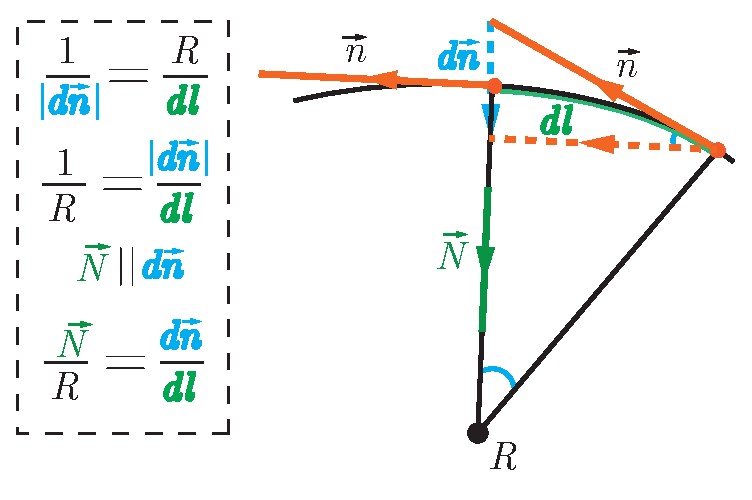
\includegraphics[width=10cm]{8.eps} %ширина рисунка составляет половину от ширины текста, picture1 - название файла с изображением, помещенного в папку Images
	\label{fig::7}
\end{figure}
\begin{figure}[h!] 	% Окружение для вставки иллюстрации
	\centering 		% Выравнивание по центру
	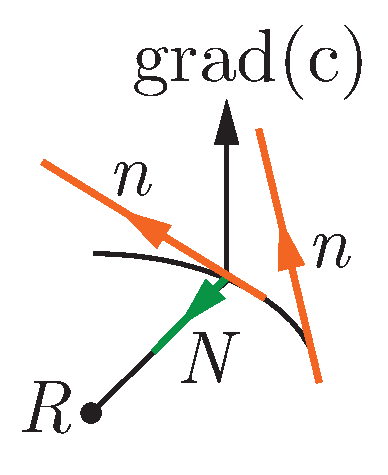
\includegraphics[width=5cm]{7.eps} %ширина рисунка составляет половину от ширины текста, picture1 - название файла с изображением, помещенного в папку Images
	\label{fig::8}
\end{figure}
где $ R $ - радиус кривизны, $ \vec{N}  $ -единичный вектор направленный к центру окружности, или по другому единичный вектор главной нормали.

Умножим \ref{66} на $ \vec{N}  $ скалярно:
\begin{equation*}
\frac{\vec{N} \vec{N} }{R} = \frac{1}{R} = \vec{N}(...)_{\text{ортогональны = 0}} - \frac{\vec{N} \nabla c }{c}
\end{equation*}

То есть луч всегда завернёт туда, где скорость звука меньше. 

\textit{Вывод:} Луч искривляется в сторону уменьшения скорости звука.

Найдём распределение звука (интенсивности) в пространстве.
$ E $ - плотность энергии звуковой волны, в общем случае, это функция координат.

Там где звука нет $ div\vec{q} = 0 $, так как 
\begin{equation*}
\dif{E}{t} + div(p\:'\vec{v}) = 0 
\end{equation*}
при отсутствии звука $ \dif{E}{t} = 0 $, $ \vec{q} $ - плотность потока энергии звуковой волны.
Используя уравнение для плоской волны:
\begin{equation*}
\vec{q} = E c \vec{n},
\end{equation*}
где $ \vec{n} $ единичный вектор вдоль $ \vec{k} $; $ \vec{k} = \nabla \psi  $ (Градиент Эйконала).

\begin{equation*}
div(E c \vec{n} ) = div(E c \frac{\vec{k}}{k} ) = div(E c \frac{\nabla\psi}{|\nabla\psi|})=0
\end{equation*}
Для нахождения $ E $ необходимо вычислить Эйконал.
Эйконал - это скалярная функция, которая определяется заранее.
Подставляем Эйконал и интегрируем.
 

\begin{center}
	\textbf{ДЗ} Скорость убывает как $ c = \frac{1}{r} \:\: n(1,0,0)_{\text{в начальный момент времени}}$ показать ход луча (получить $ n_{x}\: and\: n_{y}  $) 
\end{center}

\begin{center}
	\subsection*{Групповая скорость } % Звездочка убирает нумерацию главы
	\addcontentsline{toc}{subsection}{Групповая скорость} % Добавляет Введение в Содержание
\end{center}
$ U = \dif{\omega}{\vec{k}} $ - групповая скорость.

Выясним физический смысл групповой скорости.
Для этого рассмотрим два момента времени $ t =0  $ и произвольный близкий момент времени $ t $.
Пусть в начальный момент времени волна описывается как:

\begin{equation*}
\varphi = e^{i\vec{k}\vec{r}}f(\vec{r})
\end{equation*}
Также стоит оговорится, что в начальный момент времени звуковая волна локализована в пространстве. Тогда $ f(\vec{r}) $
должен убывать при $ r \longrightarrow \infty $. $ f(\vec{r}) $ - амплитуда зависящая от координат, которая описывает волну локализованную в пространстве.
Разложим $ f(\vec{r}) $ в ряд Фурье по плоским волнам.

Каждая Фурье компонента $ \varphi_{k}\sim e^{i\vec{k}\vec{r} + i\Delta\vec{k}\vec{r}}=e^{i((\vec{x}+\Delta\vec{x})\vec{r}} $
Частота является функцией волнового числа $ (\vec{k} + \Delta\vec{k}) \:$, то есть $ \omega(\vec{k} + \Delta\vec{k}) $. Где $ \Delta\vec{k} $ - отклонение от базового.

Итак для момента времени $ t $ имеем:
\begin{equation*}
\varphi_{k}\sim exp\left\lbrace i(\vec{k} + \Delta\vec{k})\vec{r}- i\omega t\right\rbrace 
\end{equation*}

Разложим частоту вблизи базовой частоты:
\begin{equation*}
\omega(\vec{k} + \Delta\vec{k})\approx \omega(\vec{k}) +\dif{\omega}{\vec{k}}\Delta\vec{k},
\end{equation*}
 подставим это в Фурье компоненты.
\begin{equation*}
\varphi_{k}\sim exp\left\lbrace i(\vec{k} + \Delta\vec{k})\vec{r}- i\omega t - i\dif{\omega}{\vec{k}}\Delta\vec{k}t \right\rbrace 
\end{equation*}
 Ограничиваясь линейными слагаемыми получаем:
\begin{equation*}
\varphi_{k}\sim e^{i(\vec{k}\vec{r}-\omega t)} 
exp\left\lbrace i\Delta\vec{k}(\vec{r} - i\dif{\omega}{\vec{k}}t) \right\rbrace 
\end{equation*}
Собирая обратно разложение получаем потенциал в момент времени $ t $:
\begin{equation*}
\varphi = e^{i(\vec{k}\vec{r}-\omega t)} f\left(\vec{r} - i\dif{\omega}{\vec{k}}t \right) 
\end{equation*}
То есть волновой пакет за время $ t $ перемещается со скоростью $ \dif{\omega}{\vec{k}} $ на расстояние $ \dif{\omega}{\vec{k}}t $.
А групповая скорость - это скорость движения волнового цуга.

\newpage
\begin{center}
	\section*{Шестая пара 13.02.19} % Звездочка убирает нумерацию главы
	\addcontentsline{toc}{section}{Шестая пара 13.02.19} % Добавляет Введение в Содержание

	\subsection*{Распространение звука в движущейся среде} % Звездочка убирает нумерацию главы
	\addcontentsline{toc}{subsection}{Распространение звука в движущейся среде} % Добавляет Введение в Содержание
\end{center}

Рассмотрим две системы отсчёта рис(\ref{fig::9}), где $ k' $ - система отсчёта связанная с движением среды со скоростью $ \vec{U} $.
\begin{figure}[h!] 	% Окружение для вставки иллюстрации
	\centering 		% Выравнивание по центру
	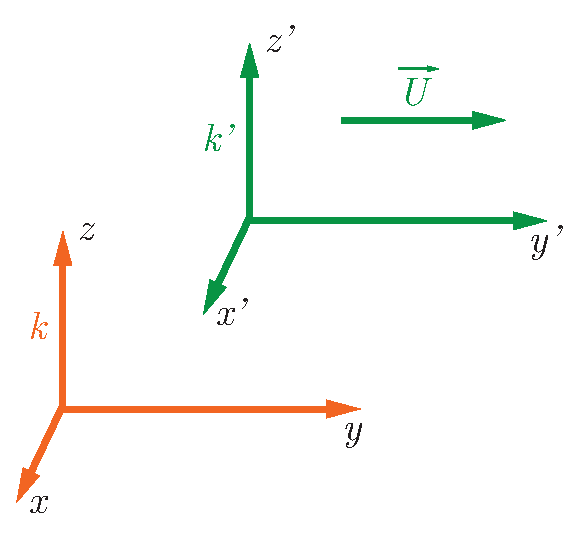
\includegraphics[width=8cm]{9.eps} %ширина рисунка составляет половину от ширины текста, picture1 - название файла с изображением, помещенного в папку Images
	\caption{Системы отсчёта}
	\label{fig::9}
\end{figure}
 
 Будем рассматривать плоскую монохроматическую волну. Поэтому имеем:
\begin{equation*}
\varphi = \varphi_{0}\;e^{i(\vec{k}\vec{r}\:'-\omega' t)}, 
\end{equation*}
где $ \omega' = ck $.  Не стоит забывать что $ k $ и $ k' $ - эквивалентны, исходя из того, что длина волны инвариантна.

Тогда выясним как будет выглядеть решение для плоской звуковой волны в лабораторной системе отсчёта.
Связь между векторами запишем следующим образом:
$ \vec{r} = \vec{r}\;'+  \vec{U}t $, или как принято у нас в колхозе $ \vec{r}\;' = \vec{r}  -  \vec{U}t $. Тогда для лабораторной системы отсчёта будем иметь:
\begin{equation*}
\varphi = \varphi_{0}e^{i(\vec{k}\vec{r}-(\vec{k}\vec{U}+\omega') t)}.
\end{equation*}
И если это выражение интерпретировать, как выражение плоской монохроматической волны, то $ (\vec{k}\vec{U}+\omega') $ должно иметь смысл частоты. $ \omega = ck + \vec{k}\vec{U} $ и от сюда мы видим, что частота не является инвариантом, она плывёт, течёт и всё такое прочее.

Скорость распространения волны представляет собой следующее:
\begin{equation*}
\diff{\omega}{\vec{k}} = c \frac{\vec{k}}{k} + \vec{U}, \;\;\;\nabla r = \frac{\vec{r}}{r}
\end{equation*}
это геометрическая скорость звука $ c $ в направлении $ \vec{k} $ и снос скорости $ \vec{U} $
Из этого выражения видно, что частота волны может и возрастать или убывать в зависимости от направления   $ \vec{k} $ и $ \vec{U} $.

Эффект изменения частоты в зависимости от скорости движения источника получил название - \textit{Эффекта Доплера}.
Он заключается в том, что частота звука воспринимаемая наблюдателем движущимся относительно источника не совпадает с частотой в неподвижной системе координат.
Если вычислим скалярное произведение (рис.\ref{fig::10}) получим следующее:

\begin{figure}[h!] 	% Окружение для вставки иллюстрации
	\centering 		% Выравнивание по центру
	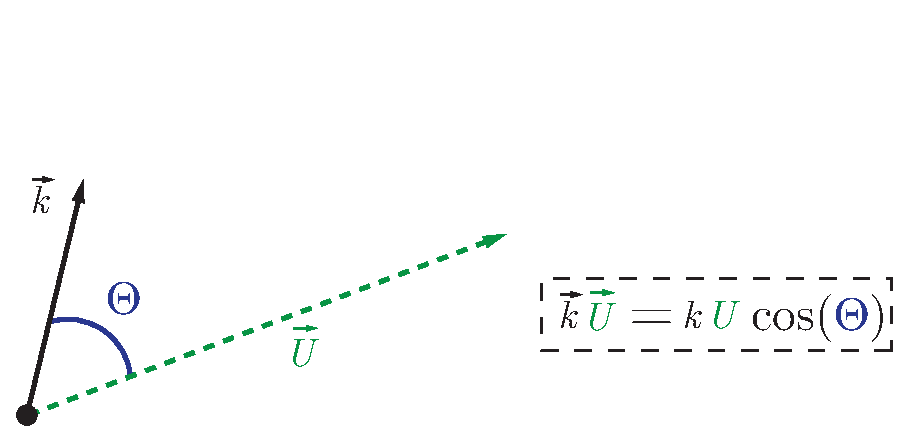
\includegraphics[width=12cm]{10.eps} %ширина рисунка составляет половину от ширины текста, picture1 - название файла с изображением, помещенного в папку Images
	\caption{Скалярное произведение}
	\label{fig::10}
\end{figure}

\begin{equation*}
\omega = \omega'\left( 1- \frac{U}{c}\cos \Theta\right),
\end{equation*}
конечно, и индусу ясно, что $ \left(\frac{U}{c}\cos\Theta\right) $ - это скорость источника.


\begin{center}
		\subsection*{Сферические волны} % Звездочка убирает нумерацию главы
\addcontentsline{toc}{subsection}{Сферические волны} % Добавляет Введение в Содержание
\end{center}
Рассмотрим звуковую волну в которой распределение плотности, давления и другие зависят только от расстояния до некоторой точки. Пусть эта звуковая волна обладает сферической симметрией.
Уравнение звуковых незатухающей волны имеет стандартный вид:

 \begin{equation*}
\Delta\varphi - \frac{1}{c^{2}}\dif{^{2}\varphi}{t^{2}} = 0
 \end{equation*}
Работать будем в сферических координатах $ \dif{}{\alpha} = 0 $ и $ \dif{}{\theta} = 0 $ это вытекает для случая симметрии.

Тогда получаем:
\begin{equation*}
\dif{^{2}\varphi}{t^{2}} =  \frac{c^{2}}{r^{2}}\frac{\partial }{\partial r}\left(r^{2} \dif{\varphi}{r}\right)  = 0,
\end{equation*}
Для тех кто в танке это волновое уравнение с учётом симметрии, как бы лаплас без занулившихся слагаемых (ну или по-научному с учётом особенностей в начале координат).
Решение будем искать в виде $ \varphi =\frac{f(r,t)}{r} $.
\begin{equation*}
\frac{\partial^{2} }{\partial t^{2}} \frac{f(r,t)}{r} = \frac{c^{2}}{r^{2}}\frac{\partial }{\partial r}r^{2}\frac{\partial }{\partial r}\frac{f(r,t)}{r} = \frac{c^{2}}{r^{2}}\frac{\partial }{\partial r}r^{2}\left(\frac{f'}{r} - \frac{f(r,t)}{r^{2}} \right)  
\end{equation*}
\begin{equation*}
\frac{1}{r}\frac{\partial^{2}f }{\partial t^{2}} = \frac{c^{2}}{r^{2}}\frac{\partial }{\partial r}\left(f'r - f \right) = \frac{c^{2}}{r^{2}}(f'+rf''-f')=\frac{c^{2}}{r^{2}}rf''
\end{equation*}

\begin{equation*}
\frac{\partial^{2}f }{\partial t^{2}} = c^{2}\left(\frac{\partial^{2}f }{\partial r^{2}} \right) 
\end{equation*}
А решение этого выражения известно и представляет собой (\ref{29}):
\begin{equation*}
f = f_{1}(ct-r) + f_{2}(ct+r).
\end{equation*}
Тогда 
\begin{equation*}
\varphi = \frac{f_{1}(ct-r)}{r} + \frac{f_{2}(ct+r)}{r},
\end{equation*}
где первому отвечает расходящаяся волна, а второму сходящаяся волна. Нужно оговориться, что сходящиеся и расходящиеся волны - это принципиально разные волны.
Отсюда ясно наблюдается, что интенсивность волны определяющейся квадратом амплитуды убывает как $ \frac{1}{r^{2}} $.

\begin{equation*}
\dot{p} = -\rho \frac{\partial\varphi}{\partial t};\;\;\;\rho' = \frac{f}{c^{2}}\frac{\partial\varphi}{\partial t},
\end{equation*}
где $ \dot{p} $ -отклонение давления от среднего значения, $ \rho $ - полная плотность, $ \rho' $ - колебания плотности.

Распределение плотности и давления определяются теми же формулами, что и для потенциала.$ \vec{v} = \nabla\varphi $ у скорости может быть только радиальная компонента.$ v_{r} = \frac{\partial\varphi}{\partial r} $. То есть для расходящейся монохроматической волны имеем:

\begin{equation*}
\varphi  = A \frac{e^{i(\vec{k}\vec{r}-\omega t)}}{r}
\end{equation*}
И она обладает особенностями в точке $ r = 0 $. Поэтому для описания может быть полезна $ \delta $ - функция, прям как в электродинамике. Спасибо, Лифшицу за это.
Сферической симметрией может обладать и стоячая волна.
Однако её потенциал должен быть конечен при $ r = 0 $.
Тогда предыдущее решение должно упроститься, исчезнет $ \cos kr $.
\begin{equation*}
\varphi  = A e^{-i\omega t}\; \frac{\sin kr}{r},
\end{equation*}
а в пределе $ r = 0 $ получаем:
\begin{equation*}
\varphi  = A e^{-i\omega t}\;k.
\end{equation*}
Но помнить нужно об истине простой, $ r = 0 $ не является узлом стоячей волны, она лишь соответствует пучности.  

\newpage
\begin{center}
	\section*{Седьмая пара 20.02.19} % Звездочка убирает нумерацию главы
	\addcontentsline{toc}{section}{Седьмая пара 20.02.19} % Добавляет Введение в Содержание
	
	\subsection*{Цилиндрические волны} % Звездочка убирает нумерацию главы
	\addcontentsline{toc}{subsection}{Цилиндрические волны} % Добавляет Введение в Содержание
\end{center}

\begin{figure}[h!] 	% Окружение для вставки иллюстрации
	\centering 		% Выравнивание по центру
	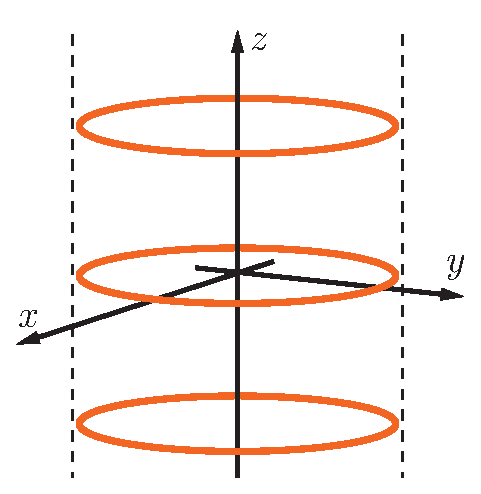
\includegraphics[width=7cm]{11.eps} %ширина рисунка составляет половину от ширины текста, picture1 - название файла с изображением, помещенного в папку Images
\end{figure}

Сформулируем задачу в терминах потенциалов скорости.
В цилиндрической системе координат решение для волны как и ранее обладает осе симметрией и поэтому в уравнении Лапласа остаётся только радиальная часть:  
\begin{equation*}
	\frac{1}{r}\frac{\partial }{\partial r}\left(r\frac{\partial \varphi}{\partial r} \right) - \frac{1}{c^{2}}\frac{\partial^{2} \varphi}{\partial t^{2}} = 0.
\end{equation*}
Это уравнение описывает бездисперсионные волны. Решение будем искать в виде $ \varphi = e^{-i\omega t}\:f(r)  $, стоит также оговориться, что волна является монохроматической. Подставляя в выражение имеем:
\begin{equation*}
e^{-i\omega t}\frac{1}{r}\frac{\partial }{\partial r}\left(r\frac{\partial f(r)}{\partial r} \right) - e^{-i\omega t}\frac{1}{c^{2}}f(r) \omega^{2},
\end{equation*}
 учитывая, что $ \frac{\omega^{2}}{c^{2}} = k^{2} $, мы так ввели.
 Получим уравнение описывающее пространственную часть:
 \begin{equation*}
f''+\frac{1}{r}f'+k^{2}f^{2}=0.
 \end{equation*}
Оно, конечно известно для мат.физики. И представляет собой функцию Бесселя нулевого порядка (рис.\ref{fig::11}).
\begin{figure}[h!] 	% Окружение для вставки иллюстрации
	\centering 		% Выравнивание по центру
	\includegraphics[width=10cm]{BS.png} %ширина рисунка составляет половину от ширины текста, picture1 - название файла с изображением, помещенного в папку Images
	\caption{Функция Бесселя}
	\label{fig::11}
\end{figure}
Для начала выясним как будет выглядеть решение в случае стоячей волны при $ r = 0, \;\varphi  $ - остаётся конечной. В итоге решением будет функция Бесселя \RomanNumeralCaps{1} го рода $ J_{0}(kr) $.
Для стоячей волны имеем следующее решение:
 \begin{equation*}
\varphi = A e^{-i\omega t}\:J_{0}(kr).
\end{equation*}
 
Из справочника Корна на больших расстояниях имеем следующее выражение:
\begin{equation*}
J_{m}(z) \approx \sqrt{\frac{2}{\pi z}}\left[A_{m}(z)cos\left(z - \frac{m\pi}{2} - \frac{\pi}{4} \right) - B_{m}(z)\sin\left(z - \frac{m\pi}{2} - \frac{\pi}{4} \right)   \right],
\end{equation*}
\begin{equation*}
A_{m}(z)  \approx  1 - \frac{(4m^{2}-1)(4m^{2}-9)}{2!(8z)^{2}} + ...\;,
\end{equation*}
\begin{equation*}
B_{m}(z)  \approx  \frac{(4m^{2}-1)}{8z} - ...\;.
\end{equation*}
при $ z \longrightarrow 0 ,\; A_{m}(z) \longrightarrow 1,\; B_{m}(z) \longrightarrow 0 $, тогда:
\begin{equation*}
 J_{0}(z) = \sqrt{\frac{2}{\pi z}}\cos\left(z - \frac{\pi}{4} \right) \Rightarrow
\end{equation*}
\begin{equation*}
\varphi = A\sqrt{\frac{2}{\pi z}}\frac{\cos\left(z - \frac{\pi}{4} \right) }{\sqrt{kr}}e^{-i\omega t},
\end{equation*}
полученное решение оговоримся применимо на больших расстояниях. Амплитуда убывает как $ \frac{1}{\sqrt{r}} $.
Вот и различие с сферическими там сразу синус, а тут Бессель всё не так убывает, + различие в интенсивности и амплитуде $  (\text{интенсивность} = \text{амплитуда}^{2}) $

Решение для расходящейся (бегущей волны) имеет вид:
\begin{equation*}
\varphi = A e^{-i\omega t}\:H_{0}^{1}(kr),
\end{equation*}
где $ H_{0}^{1} $ - функция Ханкеля \RomanNumeralCaps{1} го рода.
\begin{figure}[h!] 	% Окружение для вставки иллюстрации
	\centering 		% Выравнивание по центру
	\includegraphics[width=10cm]{NM.eps} %ширина рисунка составляет половину от ширины текста, picture1 - название файла с изображением, помещенного в папку Images
	\caption{Функция Неймана}
	\label{fig::12}
\end{figure}
 
\begin{equation*}
 H_{m}^{1} = J_{m} + iN_{m},
\end{equation*}
$ J_{m}  $ - конечно, $ N_{m} $ - расходится при $ r = 0 $, а называется функцией Неймана (рис.\ref{fig::12}).
При $ z \longrightarrow 0  $ 

\begin{equation*}
H_{0}^{1} \sim \frac{2i}{\pi}\ln\frac{z}{2},
\end{equation*}
то есть пренебрегаем $ J_{m} $ и тогда результирующий потенциал:
 \begin{equation*}
 \varphi = Ae^{-i\omega t}\left( \frac{2i}{\pi}\ln\frac{kr}{2} \right).
 \end{equation*}
На больших расстояниях, когда $ z\longrightarrow \infty $
 \begin{equation*}
H_{m}^{1}(z) = \sqrt{\frac{2}{\pi z}}e^{i\left(z - \frac{m\pi}{2} - \frac{\pi}{4} \right) }, \text{так как m = 0}
\end{equation*}
получаем для потенциала следующее:
\begin{equation*}
\varphi = A\sqrt{\frac{2}{\pi}}\frac{e^{i\left(kr - \omega t - \frac{\pi}{4}\right) }}{\sqrt{kr}}.
\end{equation*}
На больших расстояниях амплитуда цилиндрической волны падает по закону  $ \frac{1}{\sqrt{r}} $. То есть также как и у стоячей волны. То есть сферическую и цилиндрическую волну можно различить.

\begin{center}
	\subsection*{Боковая волна} % Звездочка убирает нумерацию главы
\addcontentsline{toc}{subsection}{Боковая волна} % Добавляет Введение в Содержание
\end{center}

\begin{figure}[h!] 	% Окружение для вставки иллюстрации
	\centering 		% Выравнивание по центру
	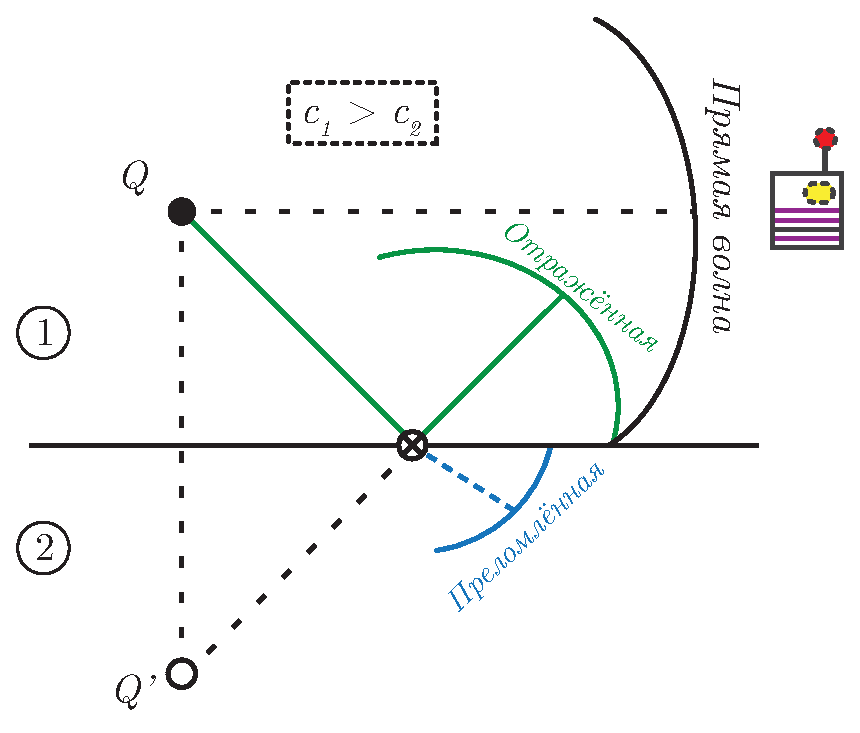
\includegraphics[width=10cm]{12.eps} %ширина рисунка составляет половину от ширины текста, picture1 - название файла с изображением, помещенного в папку Images
	\caption{$ c_{1} > c_{2} $}
	\label{fig::13}
\end{figure}

Рассмотрим задачу с границей раздела (рис.\ref{fig::13}).
Области $ 1 $ и $ 2 $ - разные среды, $ Q $ - точечный источник сферической звуковой волны, $ Q' $ - зеркальное изображение источника.
Например звук из стекла в воздух (особенность звука как мы помним, если не помним, вспомни!).
Таким образом фронт волны - это отражённая волна от источника.
Граница раздела  - это граница в которой существует несколько решений.
Но если поставим приёмник, то сначала в приёмник придёт прямая волна, потом отражённая.

Рассмотрим задачу с границей раздела (рис.\ref{fig::14}).
\begin{figure}[h!] 	% Окружение для вставки иллюстрации
	\centering 		% Выравнивание по центру
	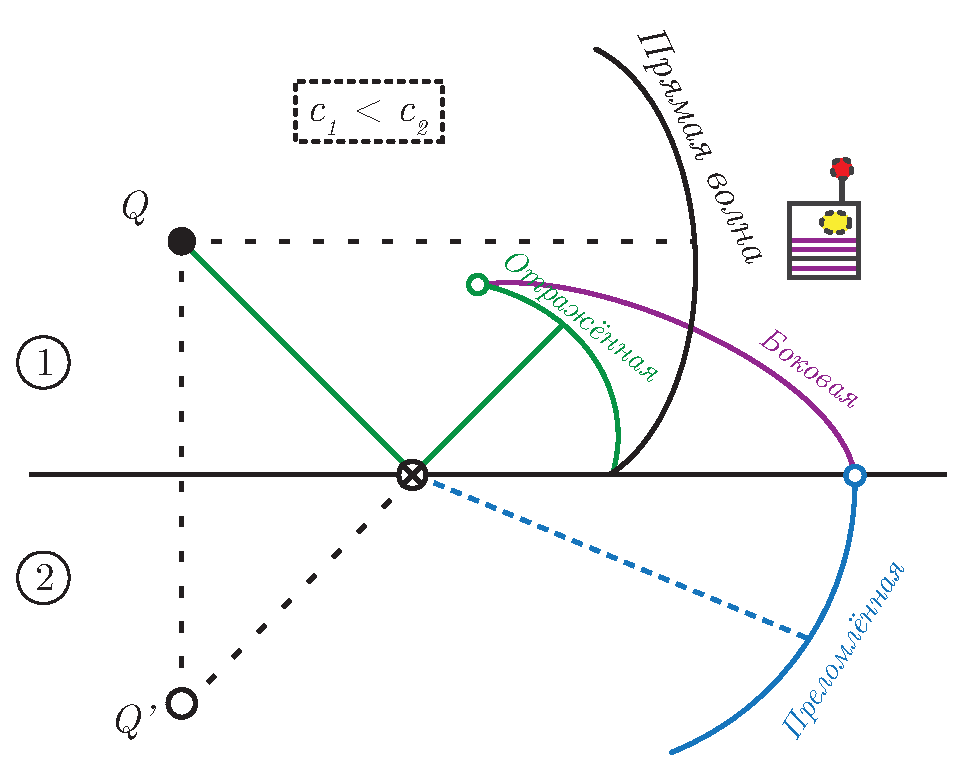
\includegraphics[width=14cm]{13.eps} %ширина рисунка составляет половину от ширины текста, picture1 - название файла с изображением, помещенного в папку Images
	\caption{$ c_{1} < c_{2} $}
	\label{fig::14}
\end{figure}
Видно, что создаётся необычное явление, а именно боковая волна.

\begin{center}
	\subsection*{Поглощение звука} % Звездочка убирает нумерацию главы
	\addcontentsline{toc}{subsection}{Поглощение звука} % Добавляет Введение в Содержание
	\textit{ Формула Киргофа }
\end{center}

Учтём теперь наличие у среды вязкости и теплопроводности. И рассмотрим такую среду по отношению к акустическим волнам.
И индюку ясно, что вязкость и теплопроводность приводит к потере энергии звуковых волн.

В истории сначала Стокс рассмотрел вязкость. А потом Киргоф добавил теплопроводность и теплопроводность оказалась порядка влиянию вязкости.

Будем интересоваться $ \dot{E}_{mek} $ - диссипируемой за единицу времени механической энергией.
\begin{equation*}
E_{mek} = E_{0} - E(S),
\end{equation*}
где $ E_{0} $ - начальная энергия, $ E(S) $ - энергия тела в конечном состоянии с энтропией $ S $, которая была вначале.

Максимальная работа совершаемая  системой, когда система переходит в конечное состояние обратимым образом, через равновесное состояние с неизменной энтропией $ S $.
\begin{equation*}
\dot{E}_{mek} = - \dot{E}(S) = \frac{\partial E}{\partial S}\dot{S}\:\longrightarrow\: \frac{\partial E}{\partial S} = T \:\longrightarrow\: dE = TdS - pdV  \:\longrightarrow\: \dot{E}_{mek} = - TS.
\end{equation*}

\begin{equation*}
\dot{S} = \frac{\kappa}{T^{2}}\int\left(\nabla T \right)^{2}dV + \frac{\eta}{2T}\int\left(\frac{\partial v_{i}}{\partial x_{k}} + \frac{\partial v_{k}}{\partial x_{i}} -\frac{2}{3}\delta_{ik}\frac{\partial v_{l}}{\partial x_{l}} \right)^{2}dV + \frac{\xi}{T} \int div(\vec{v})^{2}dV,
\end{equation*}
Первое слагаемое отвечает за изменение энтропии за счёт теплопроводности, второе с третьим за изменение энтропии за счёт внутреннего трения.$ \kappa $ - Коэффициент теплопроводности, $ \eta $ - коэффициент динамической вязкости, $ \xi  $ - коэффициент объёмного трения.
Эта формула демонстрирует за счёт каких механизмов может меняться энтропия рассматриваемого объёма жидкости.

Применим для плоской одномерной волны. 
\begin{equation*}
v_{x} = v_{0} \cos (kx - \omega t),\;\;\;\; v_{y} =0,\;\;\;\; v_{z} = 0.
\end{equation*}
Подставим в выражение:
\begin{equation*}
\frac{\eta}{2}\int\int \left(\eta - \frac{2}{3} \right)^{2}\left[\left(\frac{\partial v_{x}}{\partial x} \right)^{2} + \frac{4}{3}\left(\frac{\partial v_{x}}{\partial x} \right)^{2} + \frac{4}{3}\left(\frac{\partial v_{x}}{\partial x} \right)^{2}  \right]dV + \xi\left(\frac{\partial v_{x}}{\partial x} \right)^{2}dV =
\end{equation*}
\begin{equation*}
= \frac{\eta}{2}\int \frac{16+8}{9}\left(\frac{\partial v_{x}}{\partial x} \right)^{2}dV +\xi\int\left(\frac{\partial v_{x}}{\partial x} \right)^{2}dV = \left(\frac{4}{3}\eta + \xi \right) \int\left(\frac{\partial v_{x}}{\partial x} \right)^{2}dV
\end{equation*}

\begin{equation*}
T_{ij}T_{ij} = T_{11}T_{11} + T_{22}T_{22} + T_{33}T_{33}
\end{equation*}


\begin{equation*}
\frac{\partial v_{x}}{\partial x} = -v_{0}k\sin(kx-\omega t)
\end{equation*}
\begin{equation*}
\int\sin^{2}(kx-\omega t)dV = \frac{1}{2}V_{0},
\end{equation*}
среднее значение от $  \sin^{2}  = \frac{1}{2} $, $ V_{0} $ - объём среды.
В результате имеем:
\begin{equation*}
\frac{1}{2}v_{0}^{2}k^{2}V_{0}\left( \frac{4}{3}\eta + \xi\right),
\end{equation*}
$ v_{0} $ - амплитуда скорости.\\
Это вклад в полное изменение энтропии от вязких сил трения.

\newpage
\begin{center}
	\section*{Восьмая пара 27.02.19} % Звездочка убирает нумерацию главы
	\addcontentsline{toc}{section}{Восьмая пара 27.02.19} % Добавляет Введение в Содержание
\end{center}

Перейдём к температуре:
\begin{equation*}
\frac{\partial T}{\partial x} = \frac{\partial T}{\partial v}\frac{\partial v}{\partial x} = \frac{c\beta T}{C_{p}}\frac{\partial v}{\partial x} = \frac{c\beta T}{C_{p}}\left(-v_{0}k\sin(kx-\omega t) \right),
\end{equation*}
усредняя и интегрируя по $ V $ получим:
\begin{equation*}
\int \left( \nabla T\right)^{2}dV = \frac{c^{2}\beta^{2}T^{2}}{C_{p}^{2}}v_{o}^{2}k^{2}\frac{1}{2}V_{0}.
\end{equation*}
Множитель связан $ T' = \frac{c\beta Tv}{C_{p}} \longrightarrow \frac{\partial T}{\partial v} =  \frac{c\beta T}{C_{p}} $

Базовым является, что диссипация механической энергии представляет собой $ \dot{E}_{mek} = -TS $.
Энтропия определяет всю совокупность диссипативных событий.
\begin{equation*}
\dot{E}_{mek} = -T\left\lbrace\frac{\kappa}{T^{2}} \frac{c^{2}\beta^{2}T^{2}}{2C_{p}^{2}}v_{0}^{2}k^{2}V_{0}+\frac{1}{T}\left( \frac{4}{3}\eta + \xi\right)\frac{v_{0}^{2}k^{2}V_{0}}{2} \right\rbrace = 
\end{equation*}
\begin{equation}\label{68}
 =-\frac{v_{0}^{2}k^{2}V_{0}}{2}\left[\left( \frac{4}{3}\eta + \xi\right) + \frac{\kappa c^{2}\beta^{2}T}{C_{p}^{2}} \right].
\end{equation}

Для воздуха $ \eta \sim 10^{-5}  $, а $ \frac{\kappa c^{2}\beta^{2}T}{C_{p}^{2}} \sim 10^{-5}$.
Вспомнив уравнение для энергии:
\begin{equation*}
\int \overline{E}dV = \int \rho_{0}\overline{v^{2}}dV.
\end{equation*}
\begin{equation*}
\overline{E} = \frac{\rho_{0}v_{0}^{2}}{2}V_{0},
\end{equation*}
полная энергия звуковой волны с амплитудой $ v_{0} $, разделив на $ \rho $ получим:
\begin{equation*}
\frac{\overline{E}}{\rho} = \frac{v_{0}^{2}V_{0}}{2},
\end{equation*}
его подставляем в (\ref{68}) заменяя $ v_{0}^{2} $ и получаем:
\begin{equation*}
\dot{E}_{mek} = -\left[\left( \frac{4}{3}\eta + \xi\right) + \frac{\kappa c^{2}\beta^{2}T}{C_{p}^{2}} \right] \frac{k^{2}}{\rho_{0}}\overline{E} = -2\gamma c \overline{E}.
\end{equation*}
То есть механическая энергия может только убывать с течением времени. По закону $ e^{-2\gamma x} $, амплитуда убывает по закону $ e^{-\gamma x} = e^{-\gamma ct} $. $ t = \frac{x}{c}, $ где $ x $ - координата. Это получается при интегрировании $ \dot{E}_{mek} = -2\gamma c \overline{E} $.

$ \gamma $ - показывает как убывает амплитуда волны при удалении, коэффициент затухания (P.S $ k = \frac{\omega}{c}  $).
\begin{equation*}
\gamma = \frac{k^{2}}{2c\rho_{0}} \left[\left( \frac{4}{3}\eta + \xi\right) + \frac{\kappa c^{2}\beta^{2}T}{C_{p}^{2}} \right] = \frac{\omega^{2}}{2c^{3}\rho_{0}}\left[\left( \frac{4}{3}\eta + \xi\right) + \frac{\kappa c^{2}\beta^{2}T}{C_{p}^{2}} \right],
\end{equation*}
коэффициент затухания акустической волны, ну и $ k $ - как все догадались волновое число.

Для голоса $ \gamma \sim 10^{-7} $, то есть значение мало. Оказывается, что звук далеко не слышен не из-за вязкости, а от чего-то другого. 

\begin{equation*}
\gamma =  \frac{\omega^{2}}{2c^{3}\rho_{0}}\left[\left( \frac{4}{3}\eta + \xi\right) + \frac{\kappa c^{2}\beta^{2}T}{C_{p}^{2}} \right],
\end{equation*}
\textit{ формула Киргофа}, а слагаемые в квадратных скобках блок материальных параметров.

Запишем уравнения для затухающей волны. Ну или как изменится уравнение для бегущей звуковой волны с учётом диссипации энергии?
Раньше было:

\begin{equation*}
\partial_{tt}\varphi = c^{2}\Delta\varphi, \;\; \text{Было} \;\; k = \frac{\omega}{c}.
\end{equation*}
Теперь добавим слагаемые с мнимой единицей:
\begin{equation*}
k = \frac{\omega}{c} + ia\omega^{2}, \;\; \text{где} \;\; a\omega^{2} = \gamma.
\end{equation*}
В отсутствии поглощения было (в терминах давления) $ a = \frac{1}{2c^{2}\rho_{0}}\left( \frac{4}{3}\eta + \xi\right) + \frac{\kappa c^{2} p^{2}}{C_{p}} $, $ p' = p(x - ct) $.

Факторизуем выражение:
\begin{equation*}
\frac{\partial^{2} p'}{\partial t^{2}} = c^{2}\frac{\partial^{2} p'}{\partial x^{2}},
\end{equation*}

Процесс факторизации заключается в следующем:
\begin{equation*}
\frac{\partial^{2} p'}{\partial t^{2}} = c^{2}\frac{\partial^{2} p'}{\partial x^{2}} \;\; \text{записываем в виде}
\end{equation*}
\begin{equation*}
\left( \frac{\partial}{\partial t} - c\frac{\partial}{\partial x}  \right)\left( \frac{\partial}{\partial t} + c\frac{\partial}{\partial x}  \right)p' = 0
\end{equation*}
Раскрывая получаем исходное выражение. Но тут мы можем ограничится одной скобкой, а под скобкой тут ещё понимается одна сторона, левая или правая.
В итоге для одной стороны имеем:

\begin{equation*}
\frac{\partial p'}{\partial t} = c\frac{\partial p'}{\partial x}. 
\end{equation*}
Теперь учётом диссипации $ k $ имеем другой вид решения $ e^{i(kx-\omega t)} $. Как измениться (\ref{69}) с учётом диссипации.
\begin{equation}\label{69}
\frac{\partial p'}{\partial x} = - \frac{1}{c}\frac{\partial p'}{\partial t}.
\end{equation}

\begin{equation*}
\frac{\partial p'}{\partial x} = - \frac{1}{c}\frac{\partial p'}{\partial t} + a\frac{\partial^{2} p'}{\partial t^{2}}.
\end{equation*}
\begin{equation*}
ik = \frac{1}{c}i\omega + a(i\omega)^{2} \;\;\longrightarrow\;\; k = \frac{\omega}{c} + ia\omega^{2}.
\end{equation*}

Сведём наше уравнение к мат.физике, чтоб получить одно из \RomanNumeralCaps{3}-х решаемых там уравнений.
Введём новую переменную $ \tau = t - \frac{x}{c} $.
\begin{equation*}
\frac{\partial p'}{\partial x} = \frac{\partial p'}{\partial x'}\frac{\partial x'}{\partial x} + \frac{\partial p'}{\partial \tau}\frac{\partial \tau}{\partial x} = \frac{\partial p'}{\partial x'} -\frac{1}{c} \frac{\partial p'}{\partial \tau},
\end{equation*}
где $ x' $ - новая пространственная переменная.
\begin{equation*}
\frac{\partial p'}{\partial t} = \frac{\partial p'}{\partial \tau}\frac{\partial \tau}{\partial t} + \frac{\partial p'}{\partial x}\frac{\partial x}{\partial t} = \frac{\partial p'}{\partial \tau} -\frac{1}{c} \frac{\partial p'}{\partial x}.
\end{equation*}
В итоге:
\begin{equation*}
\frac{\partial^{2} p'}{\partial t^{2}} = \frac{\partial^{2} p'}{\partial \tau^{2}}.
\end{equation*}
Подставляя, получаем: 
\begin{equation*}
\frac{\partial^{2} p'}{\partial x'} = a\frac{\partial^{2} p'}{\partial \tau^{2}}.
\end{equation*}
Мы перешли в систему отсчёта связанную с волной. Ну и как бы получили одномерное уравнение теплопроводности с инвертированными координатами.

Оказывается, что затухающая волна подобна температурной волне и описывается уравнениями теплопроводности.
И звук который мы слышим плохо затухает. И это связанно не с диссипацией, а с рассеиванием.
Вот это поворот вот.

\newpage
\begin{center}
	\subsection*{Shock wave - ударная волна} % Звездочка убирает нумерацию главы
	\addcontentsline{toc}{subsection}{Shock wave - ударная волна} % Добавляет Введение в Содержание
	Новая веха в истории.
\end{center}

\underline{Распространения возмущения в потоке сжимаемого газа - парадокс. }

Если газ подвергается возмущению, то влияние этого возмущения относительно газа, распространяется со скоростью звука, это возмущение представляет собой сферические волны. 
\begin{figure}[h!] 	% Окружение для вставки иллюстрации
	\centering 		% Выравнивание по центру
	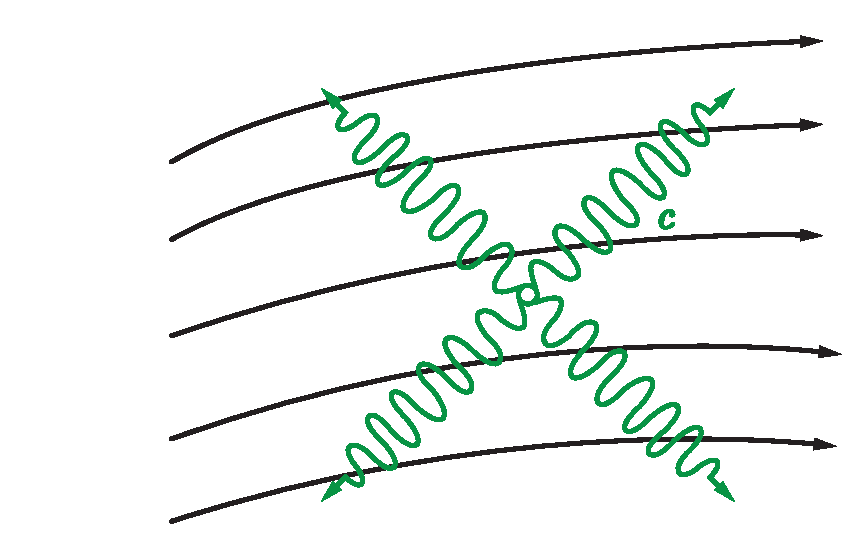
\includegraphics[width=10cm]{14.eps} %ширина рисунка составляет половину от ширины текста, picture1 - название файла с изображением, помещенного в папку Images
	\caption{Функция Неймана}
	\label{fig::15}
\end{figure}  

Пусть будет лабораторная система отсчёта относительно которой и движется среда с скоростью $ v $.
Итак, что мы будем наблюдать: 

Случай $ v<c $, вариант дозвуковых скоростей.
В дозвуковом потоке акустическая волна распространяется как вверх по потоку, так и вниз.
\begin{figure}[h!] 	% Окружение для вставки иллюстрации
	\centering 		% Выравнивание по центру
	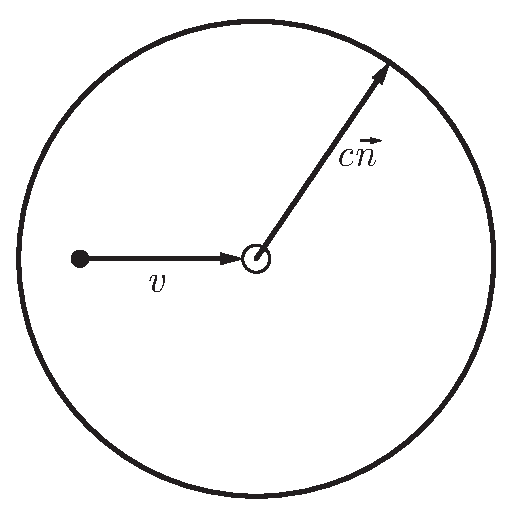
\includegraphics[width=6.5cm]{15.eps} %ширина рисунка составляет половину от ширины текста, picture1 - название файла с изображением, помещенного в папку Images
	\caption{  $ v<c $ }
	\label{fig::16}
\end{figure}

Случай $ v>c $, вариант сверхзвуковых скоростей.
\begin{figure}[h!] 	% Окружение для вставки иллюстрации
	\centering 		% Выравнивание по центру
	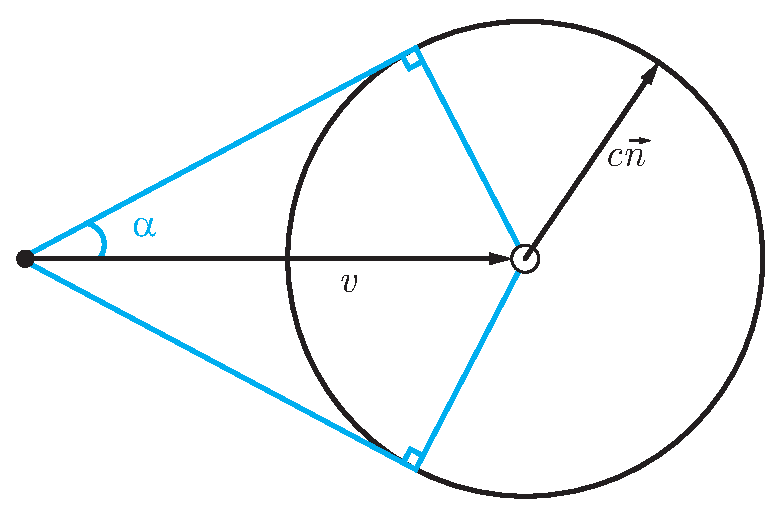
\includegraphics[width=10cm]{16.eps} %ширина рисунка составляет половину от ширины текста, picture1 - название файла с изображением, помещенного в папку Images
	\caption{  $ v>c $ }
	\label{fig::17}
\end{figure}
В сверх звуковом потоке исходящие из некоторой точки возмущения распространяются только вниз по потоку + внутри конуса с раствором:
\begin{equation*}
\sin \alpha = \frac{c}{v} \;\;\longrightarrow \alpha = \arcsin \frac{c}{v},
\end{equation*}
где $ \alpha $ - угол возмущения.

\begin{equation*}
\text{Число Маха}\:\: M = \frac{v}{c}
\end{equation*}

Поверхность ограничивающая область куда могут попасть возмущения называется характеристической.
В общем случае характеристическая поверхность не является канонической, так как скорость звука различна в разных областях газа.

Если газ обтекает препятствие с дозвуковой скоростью, то возмущение изменяется за счёт препятствия форму течения как вверх по потоку, так и вниз. Влияние этого возмущения возникает асимптотически при удалении от тела.

А сверхзвуковой поток натекает на препятствие слепо. Влияние препятствующего тела распространяется на область только вниз по течению. Во всей остальной области газ движется так, как если бы никакого препятствия не было. Под возмущением газа мы понимаем звуковую волну. $ Re>>1 $ - для нашего случая.        
















\end{document}
